% Options for packages loaded elsewhere
% Options for packages loaded elsewhere
\PassOptionsToPackage{unicode}{hyperref}
\PassOptionsToPackage{hyphens}{url}
%
\documentclass[
  ignorenonframetext,
  aspectratio=169,
  russian,
]{beamer}
\newif\ifbibliography
\usepackage{pgfpages}
\setbeamertemplate{caption}[numbered]
\setbeamertemplate{caption label separator}{: }
\setbeamercolor{caption name}{fg=normal text.fg}
\beamertemplatenavigationsymbolshorizontal
% remove section numbering
\setbeamertemplate{part page}{
  \centering
  \begin{beamercolorbox}[sep=16pt,center]{part title}
    \usebeamerfont{part title}\insertpart\par
  \end{beamercolorbox}
}
\setbeamertemplate{section page}{
  \centering
  \begin{beamercolorbox}[sep=12pt,center]{section title}
    \usebeamerfont{section title}\insertsection\par
  \end{beamercolorbox}
}
\setbeamertemplate{subsection page}{
  \centering
  \begin{beamercolorbox}[sep=8pt,center]{subsection title}
    \usebeamerfont{subsection title}\insertsubsection\par
  \end{beamercolorbox}
}
% Prevent slide breaks in the middle of a paragraph
\widowpenalties 1 10000
\raggedbottom
\AtBeginPart{
  \frame{\partpage}
}
\AtBeginSection{
  \ifbibliography
  \else
    \frame{\sectionpage}
  \fi
}
\AtBeginSubsection{
  \frame{\subsectionpage}
}
\usepackage{iftex}
\ifPDFTeX
  \usepackage[T1]{fontenc}
  \usepackage[utf8]{inputenc}
  \usepackage{textcomp} % provide euro and other symbols
\else % if luatex or xetex
  \usepackage{unicode-math} % this also loads fontspec
  \defaultfontfeatures{Scale=MatchLowercase}
  \defaultfontfeatures[\rmfamily]{Ligatures=TeX,Scale=1}
\fi
\usepackage{lmodern}

\usefonttheme{serif} % use mainfont rather than sansfont for slide text
\ifPDFTeX\else
  % xetex/luatex font selection
  \setmainfont[Ligatures=Common,Ligatures=TeX,Scale=0.94]{IBM Plex
Serif}
  \setsansfont[Ligatures=Common,Ligatures=TeX,Scale=MatchLowercase,Scale=0.94]{IBM
Plex Sans}
  \setmonofont[Scale=MatchLowercase,Scale=0.94]{DejaVu Sans Mono}
  \setmathfont[]{STIX Two Math}
\fi
% Use upquote if available, for straight quotes in verbatim environments
\IfFileExists{upquote.sty}{\usepackage{upquote}}{}
\IfFileExists{microtype.sty}{% use microtype if available
  \usepackage[]{microtype}
  \UseMicrotypeSet[protrusion]{basicmath} % disable protrusion for tt fonts
}{}

\usepackage{color}
\usepackage{fancyvrb}
\newcommand{\VerbBar}{|}
\newcommand{\VERB}{\Verb[commandchars=\\\{\}]}
\DefineVerbatimEnvironment{Highlighting}{Verbatim}{commandchars=\\\{\}}
% Add ',fontsize=\small' for more characters per line
\usepackage{framed}
\definecolor{shadecolor}{RGB}{241,243,245}
\newenvironment{Shaded}{\begin{snugshade}}{\end{snugshade}}
\newcommand{\AlertTok}[1]{\textcolor[rgb]{0.68,0.00,0.00}{#1}}
\newcommand{\AnnotationTok}[1]{\textcolor[rgb]{0.37,0.37,0.37}{#1}}
\newcommand{\AttributeTok}[1]{\textcolor[rgb]{0.40,0.45,0.13}{#1}}
\newcommand{\BaseNTok}[1]{\textcolor[rgb]{0.68,0.00,0.00}{#1}}
\newcommand{\BuiltInTok}[1]{\textcolor[rgb]{0.00,0.23,0.31}{#1}}
\newcommand{\CharTok}[1]{\textcolor[rgb]{0.13,0.47,0.30}{#1}}
\newcommand{\CommentTok}[1]{\textcolor[rgb]{0.37,0.37,0.37}{#1}}
\newcommand{\CommentVarTok}[1]{\textcolor[rgb]{0.37,0.37,0.37}{\textit{#1}}}
\newcommand{\ConstantTok}[1]{\textcolor[rgb]{0.56,0.35,0.01}{#1}}
\newcommand{\ControlFlowTok}[1]{\textcolor[rgb]{0.00,0.23,0.31}{\textbf{#1}}}
\newcommand{\DataTypeTok}[1]{\textcolor[rgb]{0.68,0.00,0.00}{#1}}
\newcommand{\DecValTok}[1]{\textcolor[rgb]{0.68,0.00,0.00}{#1}}
\newcommand{\DocumentationTok}[1]{\textcolor[rgb]{0.37,0.37,0.37}{\textit{#1}}}
\newcommand{\ErrorTok}[1]{\textcolor[rgb]{0.68,0.00,0.00}{#1}}
\newcommand{\ExtensionTok}[1]{\textcolor[rgb]{0.00,0.23,0.31}{#1}}
\newcommand{\FloatTok}[1]{\textcolor[rgb]{0.68,0.00,0.00}{#1}}
\newcommand{\FunctionTok}[1]{\textcolor[rgb]{0.28,0.35,0.67}{#1}}
\newcommand{\ImportTok}[1]{\textcolor[rgb]{0.00,0.46,0.62}{#1}}
\newcommand{\InformationTok}[1]{\textcolor[rgb]{0.37,0.37,0.37}{#1}}
\newcommand{\KeywordTok}[1]{\textcolor[rgb]{0.00,0.23,0.31}{\textbf{#1}}}
\newcommand{\NormalTok}[1]{\textcolor[rgb]{0.00,0.23,0.31}{#1}}
\newcommand{\OperatorTok}[1]{\textcolor[rgb]{0.37,0.37,0.37}{#1}}
\newcommand{\OtherTok}[1]{\textcolor[rgb]{0.00,0.23,0.31}{#1}}
\newcommand{\PreprocessorTok}[1]{\textcolor[rgb]{0.68,0.00,0.00}{#1}}
\newcommand{\RegionMarkerTok}[1]{\textcolor[rgb]{0.00,0.23,0.31}{#1}}
\newcommand{\SpecialCharTok}[1]{\textcolor[rgb]{0.37,0.37,0.37}{#1}}
\newcommand{\SpecialStringTok}[1]{\textcolor[rgb]{0.13,0.47,0.30}{#1}}
\newcommand{\StringTok}[1]{\textcolor[rgb]{0.13,0.47,0.30}{#1}}
\newcommand{\VariableTok}[1]{\textcolor[rgb]{0.07,0.07,0.07}{#1}}
\newcommand{\VerbatimStringTok}[1]{\textcolor[rgb]{0.13,0.47,0.30}{#1}}
\newcommand{\WarningTok}[1]{\textcolor[rgb]{0.37,0.37,0.37}{\textit{#1}}}

\usepackage{longtable,booktabs,array}
\newcounter{none} % for unnumbered tables
\usepackage{calc} % for calculating minipage widths
\usepackage{caption}
% Make caption package work with longtable
\makeatletter
\def\fnum@table{\tablename~\thetable}
\makeatother
\usepackage{graphicx}
\makeatletter
\newsavebox\pandoc@box
\newcommand*\pandocbounded[1]{% scales image to fit in text height/width
  \sbox\pandoc@box{#1}%
  \Gscale@div\@tempa{\textheight}{\dimexpr\ht\pandoc@box+\dp\pandoc@box\relax}%
  \Gscale@div\@tempb{\linewidth}{\wd\pandoc@box}%
  \ifdim\@tempb\p@<\@tempa\p@\let\@tempa\@tempb\fi% select the smaller of both
  \ifdim\@tempa\p@<\p@\scalebox{\@tempa}{\usebox\pandoc@box}%
  \else\usebox{\pandoc@box}%
  \fi%
}
% Set default figure placement to htbp
\def\fps@figure{htbp}
\makeatother


% definitions for citeproc citations
\NewDocumentCommand\citeproctext{}{}
\NewDocumentCommand\citeproc{mm}{%
  \begingroup\def\citeproctext{#2}\cite{#1}\endgroup}
\makeatletter
 % allow citations to break across lines
 \let\@cite@ofmt\@firstofone
 % avoid brackets around text for \cite:
 \def\@biblabel#1{}
 \def\@cite#1#2{{#1\if@tempswa , #2\fi}}
\makeatother
\newlength{\cslhangindent}
\setlength{\cslhangindent}{1.5em}
\newlength{\csllabelwidth}
\setlength{\csllabelwidth}{3em}
\newenvironment{CSLReferences}[2] % #1 hanging-indent, #2 entry-spacing
 {\begin{list}{}{%
  \setlength{\itemindent}{0pt}
  \setlength{\leftmargin}{0pt}
  \setlength{\parsep}{0pt}
  % turn on hanging indent if param 1 is 1
  \ifodd #1
   \setlength{\leftmargin}{\cslhangindent}
   \setlength{\itemindent}{-1\cslhangindent}
  \fi
  % set entry spacing
  \setlength{\itemsep}{#2\baselineskip}}}
 {\end{list}}
\usepackage{calc}
\newcommand{\CSLBlock}[1]{\hfill\break\parbox[t]{\linewidth}{\strut\ignorespaces#1\strut}}
\newcommand{\CSLLeftMargin}[1]{\parbox[t]{\csllabelwidth}{\strut#1\strut}}
\newcommand{\CSLRightInline}[1]{\parbox[t]{\linewidth - \csllabelwidth}{\strut#1\strut}}
\newcommand{\CSLIndent}[1]{\hspace{\cslhangindent}#1}

\ifLuaTeX
\usepackage[bidi=basic,shorthands=off,provide=*]{babel}
\else
\usepackage[bidi=default,shorthands=off,provide=*]{babel}
\fi
\ifPDFTeX
\else
\babelfont{rm}[Ligatures=Common,Ligatures=TeX,Scale=0.94]{IBM Plex
Serif}
\fi
\ifLuaTeX
  \usepackage{selnolig} % disable illegal ligatures
\fi


\setlength{\emergencystretch}{3em} % prevent overfull lines

\providecommand{\tightlist}{%
  \setlength{\itemsep}{0pt}\setlength{\parskip}{0pt}}



 

\usepackage[]{csquotes}



%%% Load theme
\usetheme{Madrid}
\makeatletter
\@ifpackageloaded{caption}{}{\usepackage{caption}}
\AtBeginDocument{%
\ifdefined\contentsname
  \renewcommand*\contentsname{Содержание}
\else
  \newcommand\contentsname{Содержание}
\fi
\ifdefined\listfigurename
  \renewcommand*\listfigurename{Список иллюстраций}
\else
  \newcommand\listfigurename{Список иллюстраций}
\fi
\ifdefined\listtablename
  \renewcommand*\listtablename{Список таблиц}
\else
  \newcommand\listtablename{Список таблиц}
\fi
\ifdefined\figurename
  \renewcommand*\figurename{Рисунок}
\else
  \newcommand\figurename{Рисунок}
\fi
\ifdefined\tablename
  \renewcommand*\tablename{Таблица}
\else
  \newcommand\tablename{Таблица}
\fi
}
\@ifpackageloaded{float}{}{\usepackage{float}}
\floatstyle{ruled}
\@ifundefined{c@chapter}{\newfloat{codelisting}{h}{lop}}{\newfloat{codelisting}{h}{lop}[chapter]}
\floatname{codelisting}{Список}
\newcommand*\listoflistings{\listof{codelisting}{Листинги}}
\makeatother
\makeatletter
\makeatother
\makeatletter
\@ifpackageloaded{caption}{}{\usepackage{caption}}
\@ifpackageloaded{subcaption}{}{\usepackage{subcaption}}
\makeatother

\usepackage{bookmark}
\IfFileExists{xurl.sty}{\usepackage{xurl}}{} % add URL line breaks if available
\urlstyle{same}
% fallback for those not using the hyperref driver hyperxmp:
\makeatletter
\@ifundefined{xmpquote}{\newcommand{\xmpquote}[1]{#1}}{}
\makeatother
\hypersetup{
  pdftitle={Лабораторная работа №3. Настройка прав доступа},
  pdfauthor={Мацюк Константин Владимирович},
  pdflang={ru-RU},
  hidelinks,
  pdfcreator={LaTeX via pandoc}}


\title{\texorpdfstring{Лабораторная работа №3. Настройка прав
доступа}{Лабораторная работа №3. Настройка прав доступа}}
\subtitle{\texorpdfstring{Дисциплина: Основы администрирования
операционных
систем}{Дисциплина: Основы администрирования операционных систем}}
\author{Мацюк Константин Владимирович}
\date{}

\begin{document}
\frame{\titlepage}

\renewcommand*\contentsname{Содержание}
\begin{frame}[allowframebreaks]
  \frametitle{Содержание}
  \setcounter{tocdepth}{1}
  \tableofcontents
\end{frame}
\setcounter{tocdepth}{1}
\tableofcontents
}

\section{Цель
работы}\label{ux446ux435ux43bux44c-ux440ux430ux431ux43eux442ux44b}

\begin{frame}{Цель работы}
\begin{itemize}
\tightlist
\item
  Получение навыков настройки базовых и специальных прав доступа для
  групп пользователей в операционной системе типа Linux
\end{itemize}
\end{frame}

\section{Задание}\label{ux437ux430ux434ux430ux43dux438ux435}

\begin{frame}[fragile]{Задание}
\begin{itemize}
\tightlist
\item
  Прочитать справку \texttt{man} по командам \texttt{chgrp},
  \texttt{chmod}, \texttt{getfacl}, \texttt{setfacl}
\item
  Настроить базовые разрешения для групп пользователей, раздел 3.3.1
\item
  Настроить специальные разрешения, раздел 3.3.2
\item
  Настроить расширенные разрешения с использованием ACL, раздел 3.3.3
\end{itemize}
\end{frame}

\section{Теоретическое
введение}\label{ux442ux435ux43eux440ux435ux442ux438ux447ux435ux441ux43aux43eux435-ux432ux432ux435ux434ux435ux43dux438ux435}

\begin{frame}[fragile]{Пользователи, группы и права файлов}
\protect\phantomsection\label{ux43fux43eux43bux44cux437ux43eux432ux430ux442ux435ux43bux438-ux433ux440ux443ux43fux43fux44b-ux438-ux43fux440ux430ux432ux430-ux444ux430ux439ux43bux43eux432}
\begin{itemize}
\tightlist
\item
  Файл имеет пользователя-владельца и группу-владельца
\item
  Категории доступа: владелец \texttt{u}, группа \texttt{g}, остальные
  \texttt{o}
\item
  \texttt{r} разрешает чтение содержимого файла
\item
  \texttt{w} разрешает изменение содержимого
\item
  \texttt{x} разрешает выполнение файла
\end{itemize}
\end{frame}

\begin{frame}[fragile]{Права доступа к каталогам}
\protect\phantomsection\label{ux43fux440ux430ux432ux430-ux434ux43eux441ux442ux443ux43fux430-ux43a-ux43aux430ux442ux430ux43bux43eux433ux430ux43c}
\begin{itemize}
\tightlist
\item
  \texttt{r} позволяет получить список имён в каталоге
\item
  \texttt{x} позволяет проходить через каталог и обращаться к его
  объектам
\item
  \texttt{w} вместе с \texttt{x} позволяет создавать и удалять записи
\item
  Удаление файла определяется правами на содержащий его каталог
\end{itemize}
\end{frame}

\begin{frame}[fragile]{Восьмеричная запись прав}
\protect\phantomsection\label{ux432ux43eux441ux44cux43cux435ux440ux438ux447ux43dux430ux44f-ux437ux430ux43fux438ux441ux44c-ux43fux440ux430ux432}
\begin{itemize}
\tightlist
\item
  Чтение: \texttt{4}, запись: \texttt{2}, выполнение: \texttt{1}
\item
  \texttt{7\ =\ 4\ +\ 2\ +\ 1}, то есть \texttt{rwx}
\item
  Режим \texttt{770}: владелец и группа получают \texttt{rwx}, остальные
  не получают прав
\item
  \texttt{chgrp} изменяет группу-владельца
\item
  \texttt{chmod} изменяет разрешения
\end{itemize}

\begin{Shaded}
\begin{Highlighting}[]
\NormalTok{drwxrwx{-}{-}{-}}
\end{Highlighting}
\end{Shaded}
\end{frame}

\begin{frame}{Специальные разрешения}
\protect\phantomsection\label{ux441ux43fux435ux446ux438ux430ux43bux44cux43dux44bux435-ux440ux430ux437ux440ux435ux448ux435ux43dux438ux44f}
\begin{itemize}
\tightlist
\item
  SGID на каталоге обеспечивает наследование его группы новыми объектами
\item
  Sticky bit ограничивает удаление и переименование чужих файлов
\item
  При необходимых правах на каталог пользователь может удалить свой файл
  или файл в своём каталоге
\item
  Привилегированный пользователь может обходить ограничение sticky bit
\end{itemize}
\end{frame}

\begin{frame}[fragile]{Списки доступа ACL}
\protect\phantomsection\label{ux441ux43fux438ux441ux43aux438-ux434ux43eux441ux442ux443ux43fux430-acl}
\begin{itemize}
\tightlist
\item
  ACL задаёт разрешения дополнительным пользователям и группам
\item
  ACL доступа действует на сам объект
\item
  ACL по умолчанию наследуют новые объекты каталога
\item
  \texttt{mask::} ограничивает эффективные права группы-владельца и
  именованных записей
\item
  \texttt{getfacl} просматривает ACL, \texttt{setfacl} изменяет ACL
\end{itemize}
\end{frame}

\section{Выполнение лабораторной
работы}\label{ux432ux44bux43fux43eux43bux43dux435ux43dux438ux435-ux43bux430ux431ux43eux440ux430ux442ux43eux440ux43dux43eux439-ux440ux430ux431ux43eux442ux44b}

\begin{frame}[fragile]{Рабочая среда и исходные условия}
\protect\phantomsection\label{ux440ux430ux431ux43eux447ux430ux44f-ux441ux440ux435ux434ux430-ux438-ux438ux441ux445ux43eux434ux43dux44bux435-ux443ux441ux43bux43eux432ux438ux44f}
\begin{itemize}
\tightlist
\item
  Операционная система: Rocky Linux
\item
  Пользователи и группы созданы в предыдущей работе
\item
  \texttt{alice} и \texttt{bob} входят в группу \texttt{main}
\item
  \texttt{carol} входит в группу \texttt{third}
\item
  Для проверок \texttt{bob} не входит в \texttt{third}, а \texttt{carol}
  не входит в \texttt{main}
\end{itemize}
\end{frame}

\begin{frame}{Результаты и подтверждения}
\protect\phantomsection\label{ux440ux435ux437ux443ux43bux44cux442ux430ux442ux44b-ux438-ux43fux43eux434ux442ux432ux435ux440ux436ux434ux435ux43dux438ux44f}
\begin{itemize}
\tightlist
\item
  Команды и результаты приведены по скриншотам Rocky Linux
\item
  Нумерация 28 рисунков совпадает с отчётом
\item
  Пользователи и группы повторно не создавались
\item
  Фактические права файлов проверены по выводу терминала
\end{itemize}
\end{frame}

\begin{frame}[fragile]{Справочное описание команд}
\protect\phantomsection\label{ux441ux43fux440ux430ux432ux43eux447ux43dux43eux435-ux43eux43fux438ux441ux430ux43dux438ux435-ux43aux43eux43cux430ux43dux434}
\begin{Shaded}
\begin{Highlighting}[]
\FunctionTok{man}\NormalTok{ chgrp}
\FunctionTok{man}\NormalTok{ chmod}
\FunctionTok{man}\NormalTok{ getfacl}
\FunctionTok{man}\NormalTok{ setfacl}
\end{Highlighting}
\end{Shaded}

\begin{itemize}
\tightlist
\item
  \texttt{chgrp} меняет группу объекта, \texttt{chmod} задаёт разрешения
\item
  \texttt{getfacl} и \texttt{setfacl} входят в пакет \texttt{acl}
\end{itemize}
\end{frame}

\begin{frame}[fragile]{Базовые разрешения: создание каталогов}
\protect\phantomsection\label{ux431ux430ux437ux43eux432ux44bux435-ux440ux430ux437ux440ux435ux448ux435ux43dux438ux44f-ux441ux43eux437ux434ux430ux43dux438ux435-ux43aux430ux442ux430ux43bux43eux433ux43eux432}
\begin{itemize}
\tightlist
\item
  Пункты 1--2 раздела 3.3.1
\item
  В первом терминале открыл сеанс \texttt{root}
\end{itemize}

\begin{Shaded}
\begin{Highlighting}[]
\FunctionTok{su} \AttributeTok{{-}}
\FunctionTok{mkdir} \AttributeTok{{-}p}\NormalTok{ /data/main}
\FunctionTok{mkdir} \AttributeTok{{-}p}\NormalTok{ /data/third}
\FunctionTok{ls} \AttributeTok{{-}Al}\NormalTok{ /data}
\end{Highlighting}
\end{Shaded}

\begin{itemize}
\tightlist
\item
  Подготовил каталоги; исходные владелец и группа --- \texttt{root}
\item
  Уже при первой проверке оба каталога имели режим \texttt{770}
\end{itemize}
\end{frame}

\begin{frame}{Открытие сеанса root командой su -}
\protect\phantomsection\label{ux43eux442ux43aux440ux44bux442ux438ux435-ux441ux435ux430ux43dux441ux430-root-ux43aux43eux43cux430ux43dux434ux43eux439-su--}
\begin{figure}

\centering{

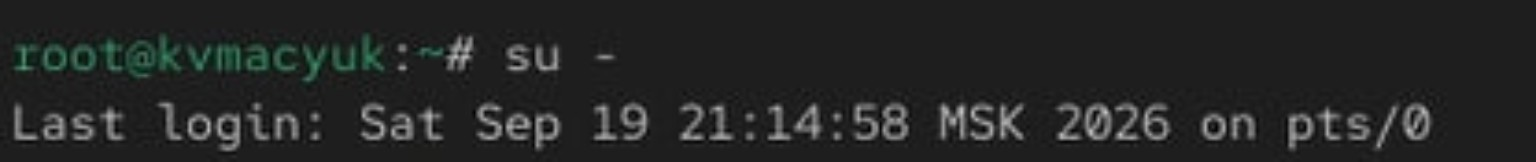
\includegraphics[width=0.85\linewidth,height=\textheight,keepaspectratio]{image/1.jpg}

}

\caption{\label{fig-001}Открытие сеанса root командой su -}

\end{figure}%
\end{frame}

\begin{frame}{Подготовка каталогов /data/main и /data/third}
\protect\phantomsection\label{ux43fux43eux434ux433ux43eux442ux43eux432ux43aux430-ux43aux430ux442ux430ux43bux43eux433ux43eux432-datamain-ux438-datathird}
\begin{figure}

\centering{

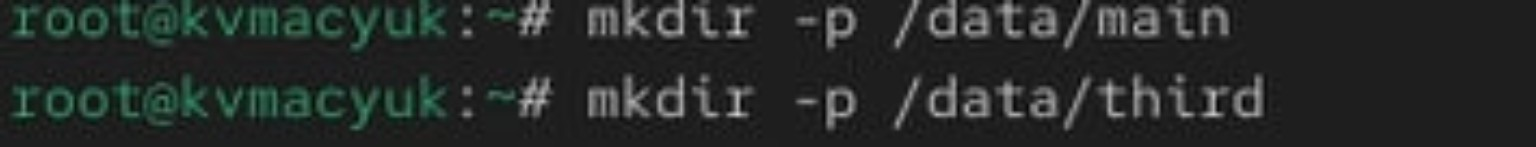
\includegraphics[width=0.85\linewidth,height=\textheight,keepaspectratio]{image/2.jpg}

}

\caption{\label{fig-002}Подготовка каталогов /data/main и /data/third}

\end{figure}%
\end{frame}

\begin{frame}{Исходные владельцы и права каталогов}
\protect\phantomsection\label{ux438ux441ux445ux43eux434ux43dux44bux435-ux432ux43bux430ux434ux435ux43bux44cux446ux44b-ux438-ux43fux440ux430ux432ux430-ux43aux430ux442ux430ux43bux43eux433ux43eux432}
\begin{figure}

\centering{

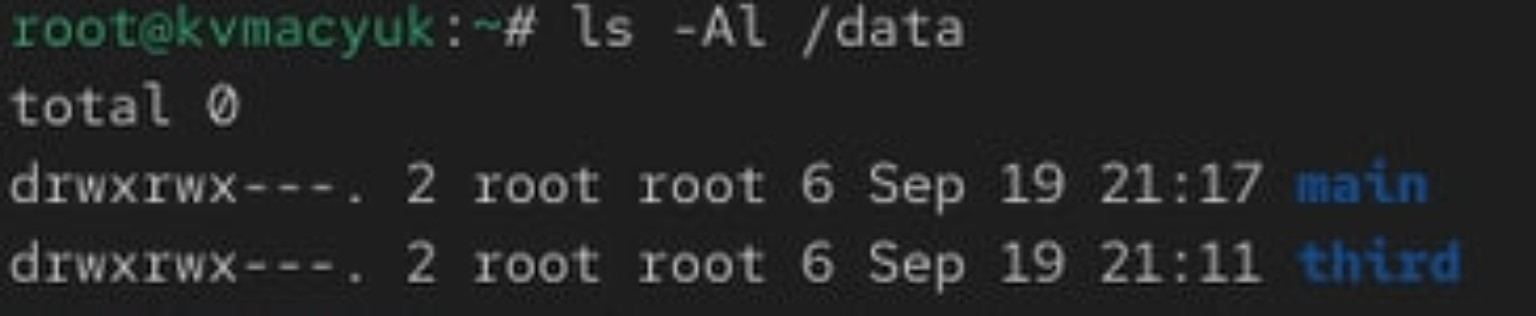
\includegraphics[width=0.85\linewidth,height=\textheight,keepaspectratio]{image/3.jpg}

}

\caption{\label{fig-003}Исходные владельцы и права каталогов}

\end{figure}%
\end{frame}

\begin{frame}[fragile]{Базовые разрешения: изменение групп}
\protect\phantomsection\label{ux431ux430ux437ux43eux432ux44bux435-ux440ux430ux437ux440ux435ux448ux435ux43dux438ux44f-ux438ux437ux43cux435ux43dux435ux43dux438ux435-ux433ux440ux443ux43fux43f}
\begin{itemize}
\tightlist
\item
  Пункт 3 раздела 3.3.1, терминал \texttt{root}
\end{itemize}

\begin{Shaded}
\begin{Highlighting}[]
\FunctionTok{chgrp}\NormalTok{ main /data/main}
\FunctionTok{chgrp}\NormalTok{ third /data/third}
\FunctionTok{ls} \AttributeTok{{-}Al}\NormalTok{ /data}
\end{Highlighting}
\end{Shaded}

\begin{itemize}
\tightlist
\item
  Группа \texttt{/data/main} становится \texttt{main}
\item
  Группа \texttt{/data/third} становится \texttt{third}
\item
  Пользователь-владелец обоих каталогов остаётся \texttt{root}
\end{itemize}
\end{frame}

\begin{frame}{Изменение групп-владельцев каталогов}
\protect\phantomsection\label{ux438ux437ux43cux435ux43dux435ux43dux438ux435-ux433ux440ux443ux43fux43f-ux432ux43bux430ux434ux435ux43bux44cux446ux435ux432-ux43aux430ux442ux430ux43bux43eux433ux43eux432}
\begin{figure}

\centering{

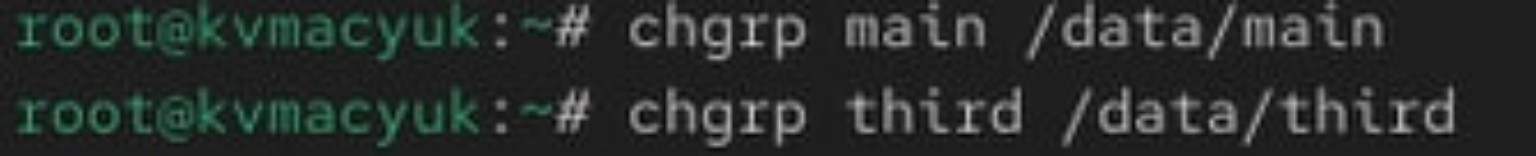
\includegraphics[width=0.85\linewidth,height=\textheight,keepaspectratio]{image/4.jpg}

}

\caption{\label{fig-004}Изменение групп-владельцев каталогов}

\end{figure}%
\end{frame}

\begin{frame}{Проверка групп main и third после chgrp}
\protect\phantomsection\label{ux43fux440ux43eux432ux435ux440ux43aux430-ux433ux440ux443ux43fux43f-main-ux438-third-ux43fux43eux441ux43bux435-chgrp}
\begin{figure}

\centering{

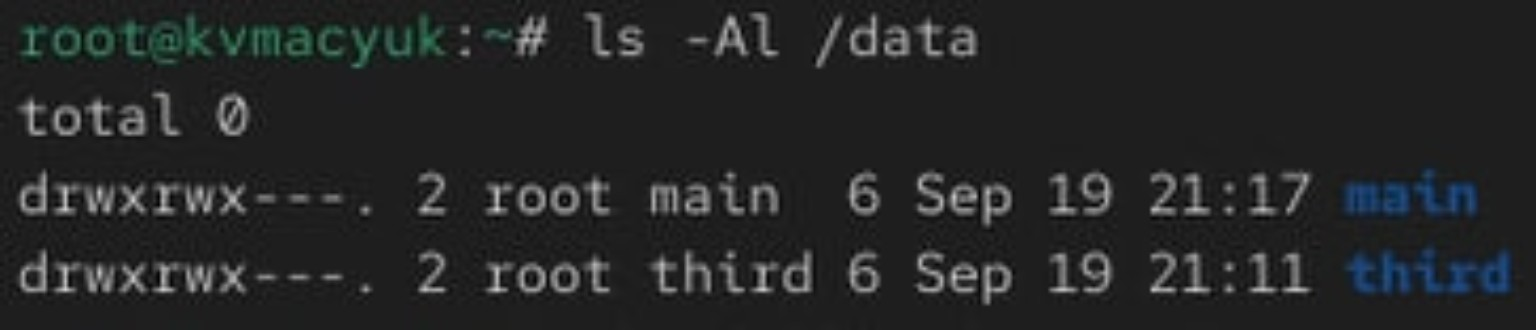
\includegraphics[width=0.85\linewidth,height=\textheight,keepaspectratio]{image/5.jpg}

}

\caption{\label{fig-005}Проверка групп main и third после chgrp}

\end{figure}%
\end{frame}

\begin{frame}[fragile]{Базовые разрешения: режим 770}
\protect\phantomsection\label{ux431ux430ux437ux43eux432ux44bux435-ux440ux430ux437ux440ux435ux448ux435ux43dux438ux44f-ux440ux435ux436ux438ux43c-770}
\begin{itemize}
\tightlist
\item
  Пункт 4 раздела 3.3.1, терминал \texttt{root}
\end{itemize}

\begin{Shaded}
\begin{Highlighting}[]
\FunctionTok{chmod}\NormalTok{ 770 /data/main}
\FunctionTok{chmod}\NormalTok{ 770 /data/third}
\FunctionTok{ls} \AttributeTok{{-}ld}\NormalTok{ /data/main /data/third}
\end{Highlighting}
\end{Shaded}

{\def\LTcaptype{none} % do not increment counter
\begin{longtable}[]{@{}llll@{}}
\toprule\noalign{}
Каталог & Владелец & Группа & Права \\
\midrule\noalign{}
\endhead
\texttt{/data/main} & \texttt{root} & \texttt{main} &
\texttt{drwxrwx-\/-\/-} \\
\texttt{/data/third} & \texttt{root} & \texttt{third} &
\texttt{drwxrwx-\/-\/-} \\
\bottomrule\noalign{}
\end{longtable}
}
\end{frame}

\begin{frame}[fragile]{Значение режима 770}
\protect\phantomsection\label{ux437ux43dux430ux447ux435ux43dux438ux435-ux440ux435ux436ux438ux43cux430-770}
\begin{itemize}
\tightlist
\item
  Владелец и соответствующая группа могут просматривать каталог и
  входить в него
\item
  Права \texttt{w} и \texttt{x} позволяют создавать и удалять записи
\item
  Остальные пользователи не получают доступа
\item
  В Rocky Linux после строки прав может стоять символ контекста
  безопасности, например точка
\item
  Этот символ не изменяет базовый режим \texttt{770}
\end{itemize}
\end{frame}

\begin{frame}{Установка и проверка режима 770}
\protect\phantomsection\label{ux443ux441ux442ux430ux43dux43eux432ux43aux430-ux438-ux43fux440ux43eux432ux435ux440ux43aux430-ux440ux435ux436ux438ux43cux430-770}
\begin{figure}

\centering{

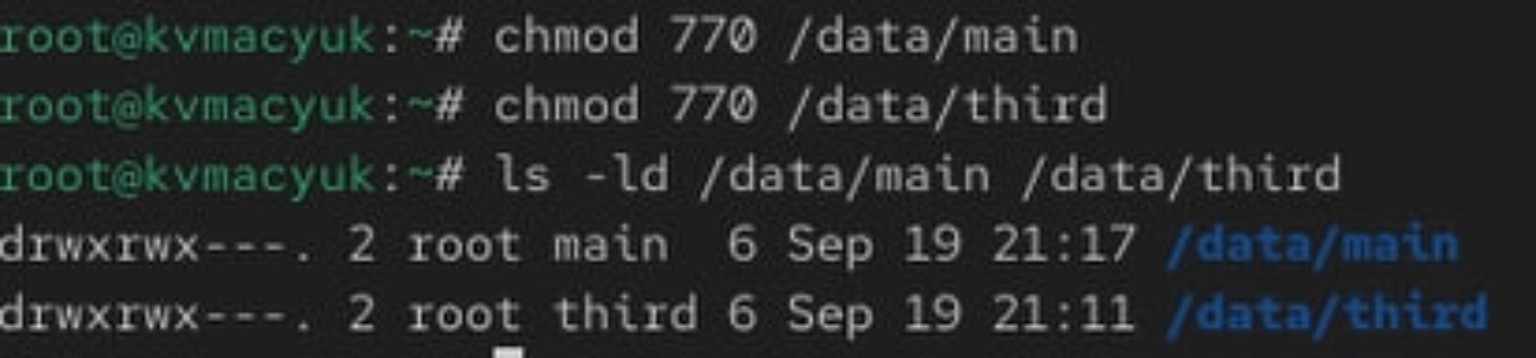
\includegraphics[width=0.85\linewidth,height=\textheight,keepaspectratio]{image/6.jpg}

}

\caption{\label{fig-006}Установка и проверка режима 770}

\end{figure}%
\end{frame}

\begin{frame}[fragile]{Пользователь bob: доступ к /data/main}
\protect\phantomsection\label{ux43fux43eux43bux44cux437ux43eux432ux430ux442ux435ux43bux44c-bob-ux434ux43eux441ux442ux443ux43f-ux43a-datamain}
\begin{itemize}
\tightlist
\item
  Пункты 5--6 раздела 3.3.1, второй терминал
\end{itemize}

\begin{Shaded}
\begin{Highlighting}[]
\FunctionTok{su} \AttributeTok{{-}}\NormalTok{ bob}
\BuiltInTok{cd}\NormalTok{ /data/main}
\FunctionTok{touch}\NormalTok{ emptyfile}
\FunctionTok{ls} \AttributeTok{{-}l}
\end{Highlighting}
\end{Shaded}

\begin{itemize}
\tightlist
\item
  Файл успешно создан: \texttt{bob} входит в \texttt{main}
\item
  Владелец и группа файла: \texttt{bob}; права: \texttt{0644}
\item
  Режим каталога в файл не копируется
\end{itemize}
\end{frame}

\begin{frame}{Переключение на пользователя bob}
\protect\phantomsection\label{ux43fux435ux440ux435ux43aux43bux44eux447ux435ux43dux438ux435-ux43dux430-ux43fux43eux43bux44cux437ux43eux432ux430ux442ux435ux43bux44f-bob}
\begin{figure}

\centering{

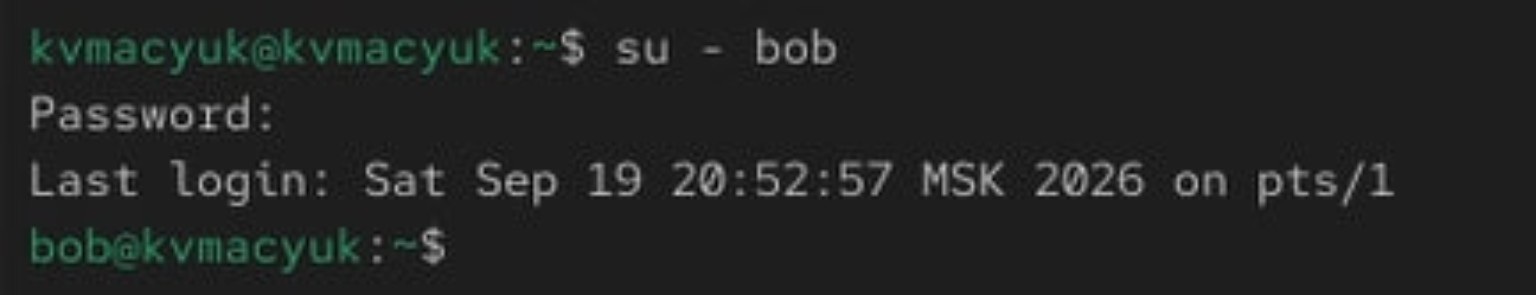
\includegraphics[width=0.85\linewidth,height=\textheight,keepaspectratio]{image/7.jpg}

}

\caption{\label{fig-007}Переключение на пользователя bob}

\end{figure}%
\end{frame}

\begin{frame}{Создание emptyfile пользователем bob}
\protect\phantomsection\label{ux441ux43eux437ux434ux430ux43dux438ux435-emptyfile-ux43fux43eux43bux44cux437ux43eux432ux430ux442ux435ux43bux435ux43c-bob}
\begin{figure}

\centering{

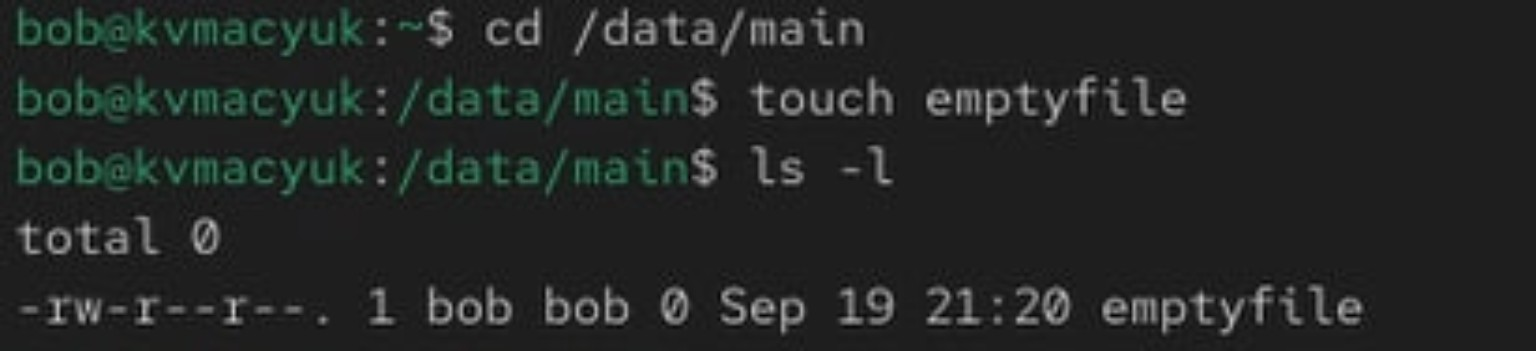
\includegraphics[width=0.85\linewidth,height=\textheight,keepaspectratio]{image/8.jpg}

}

\caption{\label{fig-008}Создание emptyfile пользователем bob}

\end{figure}%
\end{frame}

\begin{frame}[fragile]{Пользователь bob: доступ к /data/third}
\protect\phantomsection\label{ux43fux43eux43bux44cux437ux43eux432ux430ux442ux435ux43bux44c-bob-ux434ux43eux441ux442ux443ux43f-ux43a-datathird}
\begin{itemize}
\tightlist
\item
  Пункт 7 раздела 3.3.1, терминал \texttt{bob}
\end{itemize}

\begin{Shaded}
\begin{Highlighting}[]
\BuiltInTok{cd}\NormalTok{ /data/third}
\end{Highlighting}
\end{Shaded}

\begin{itemize}
\tightlist
\item
  Переход завершился сообщением \texttt{Permission\ denied}
\item
  \texttt{bob} не входит в \texttt{third}, для остальных установлено
  \texttt{-\/-\/-}
\item
  Текущим каталогом остался \texttt{/data/main}
\item
  Попытка создания файла в \texttt{/data/third} на скриншоте не показана
\end{itemize}
\end{frame}

\begin{frame}{Отказ bob в переходе в /data/third}
\protect\phantomsection\label{ux43eux442ux43aux430ux437-bob-ux432-ux43fux435ux440ux435ux445ux43eux434ux435-ux432-datathird}
\begin{figure}

\centering{

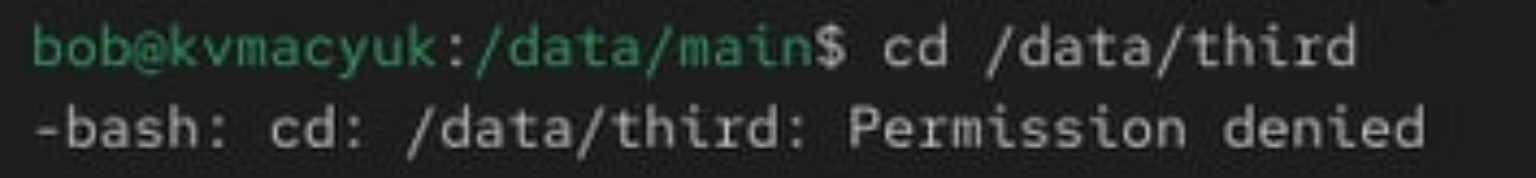
\includegraphics[width=0.85\linewidth,height=\textheight,keepaspectratio]{image/9.jpg}

}

\caption{\label{fig-009}Отказ bob в переходе в /data/third}

\end{figure}%
\end{frame}

\begin{frame}[fragile]{Специальные разрешения: файлы alice}
\protect\phantomsection\label{ux441ux43fux435ux446ux438ux430ux43bux44cux43dux44bux435-ux440ux430ux437ux440ux435ux448ux435ux43dux438ux44f-ux444ux430ux439ux43bux44b-alice}
\begin{itemize}
\tightlist
\item
  Пункты 1--2 раздела 3.3.2, новый терминал
\end{itemize}

\begin{Shaded}
\begin{Highlighting}[]
\FunctionTok{su} \AttributeTok{{-}}\NormalTok{ alice}
\BuiltInTok{cd}\NormalTok{ /data/main}
\FunctionTok{touch}\NormalTok{ alice1 alice2}
\end{Highlighting}
\end{Shaded}

\begin{itemize}
\tightlist
\item
  Создание разрешено, поскольку \texttt{alice} входит в \texttt{main}
\item
  Владелец и группа файлов \texttt{alice1} и \texttt{alice2}:
  \texttt{alice}
\end{itemize}
\end{frame}

\begin{frame}{Переключение на пользователя alice}
\protect\phantomsection\label{ux43fux435ux440ux435ux43aux43bux44eux447ux435ux43dux438ux435-ux43dux430-ux43fux43eux43bux44cux437ux43eux432ux430ux442ux435ux43bux44f-alice}
\begin{figure}

\centering{

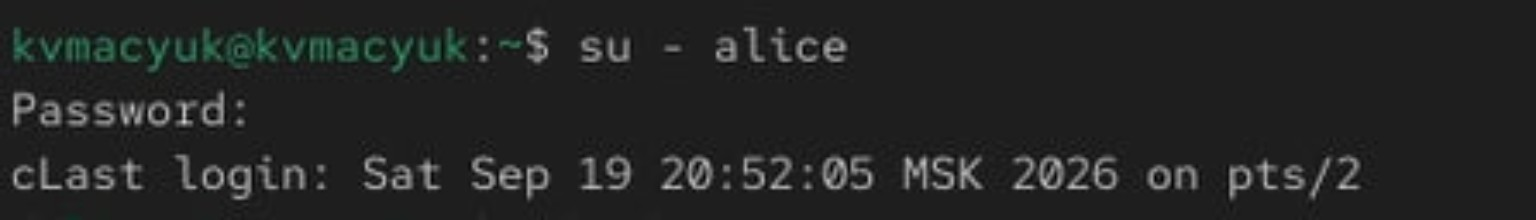
\includegraphics[width=0.85\linewidth,height=\textheight,keepaspectratio]{image/10.jpg}

}

\caption{\label{fig-010}Переключение на пользователя alice}

\end{figure}%
\end{frame}

\begin{frame}{Создание файлов alice1 и alice2}
\protect\phantomsection\label{ux441ux43eux437ux434ux430ux43dux438ux435-ux444ux430ux439ux43bux43eux432-alice1-ux438-alice2}
\begin{figure}

\centering{

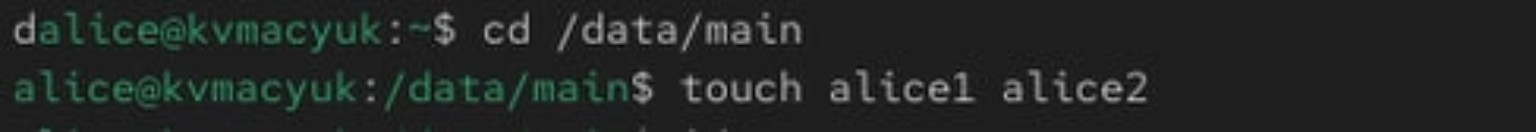
\includegraphics[width=0.85\linewidth,height=\textheight,keepaspectratio]{image/11.jpg}

}

\caption{\label{fig-011}Создание файлов alice1 и alice2}

\end{figure}%
\end{frame}

\begin{frame}[fragile]{Удаление файлов до установки sticky bit}
\protect\phantomsection\label{ux443ux434ux430ux43bux435ux43dux438ux435-ux444ux430ux439ux43bux43eux432-ux434ux43e-ux443ux441ux442ux430ux43dux43eux432ux43aux438-sticky-bit}
\begin{itemize}
\tightlist
\item
  Пункты 3--4 раздела 3.3.2, отдельный терминал \texttt{bob}
\end{itemize}

\begin{Shaded}
\begin{Highlighting}[]
\FunctionTok{ls} \AttributeTok{{-}l}
\FunctionTok{rm} \AttributeTok{{-}f}\NormalTok{ alice}\PreprocessorTok{*}
\FunctionTok{ls}
\end{Highlighting}
\end{Shaded}

\begin{itemize}
\tightlist
\item
  Файлы \texttt{alice1} и \texttt{alice2} удалились; остался
  \texttt{emptyfile}
\item
  Пользователю \texttt{bob} достаточно прав \texttt{w} и \texttt{x} на
  каталог
\end{itemize}
\end{frame}

\begin{frame}{Владельцы файлов до установки специальных битов}
\protect\phantomsection\label{ux432ux43bux430ux434ux435ux43bux44cux446ux44b-ux444ux430ux439ux43bux43eux432-ux434ux43e-ux443ux441ux442ux430ux43dux43eux432ux43aux438-ux441ux43fux435ux446ux438ux430ux43bux44cux43dux44bux445-ux431ux438ux442ux43eux432}
\begin{figure}

\centering{

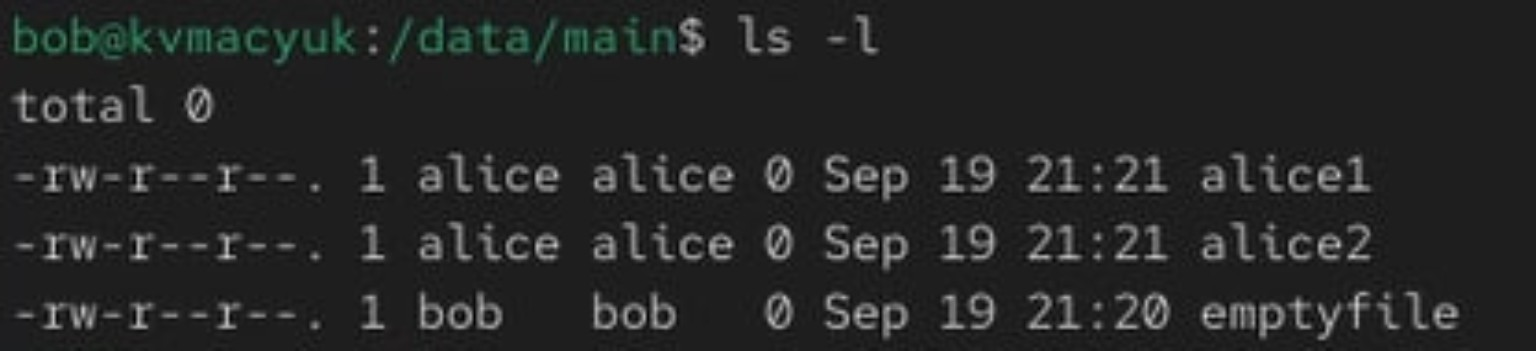
\includegraphics[width=0.85\linewidth,height=\textheight,keepaspectratio]{image/12.jpg}

}

\caption{\label{fig-012}Владельцы файлов до установки специальных битов}

\end{figure}%
\end{frame}

\begin{frame}{Удаление файлов alice1 и alice2 пользователем bob}
\protect\phantomsection\label{ux443ux434ux430ux43bux435ux43dux438ux435-ux444ux430ux439ux43bux43eux432-alice1-ux438-alice2-ux43fux43eux43bux44cux437ux43eux432ux430ux442ux435ux43bux435ux43c-bob}
\begin{figure}

\centering{

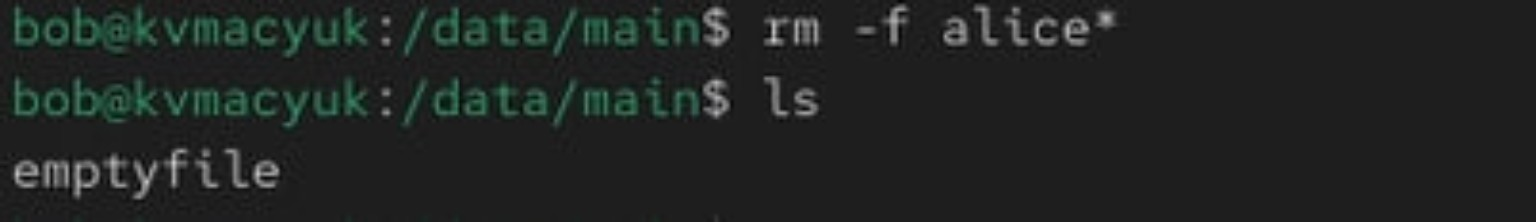
\includegraphics[width=0.85\linewidth,height=\textheight,keepaspectratio]{image/13.jpg}

}

\caption{\label{fig-013}Удаление файлов alice1 и alice2 пользователем
bob}

\end{figure}%
\end{frame}

\begin{frame}[fragile]{Создание файлов bob}
\protect\phantomsection\label{ux441ux43eux437ux434ux430ux43dux438ux435-ux444ux430ux439ux43bux43eux432-bob}
\begin{itemize}
\tightlist
\item
  Пункт 5 раздела 3.3.2, тот же терминал \texttt{bob}
\end{itemize}

\begin{Shaded}
\begin{Highlighting}[]
\FunctionTok{touch}\NormalTok{ bob1 bob2}
\FunctionTok{ls} \AttributeTok{{-}l}
\end{Highlighting}
\end{Shaded}

\begin{itemize}
\tightlist
\item
  Владелец и группа обоих файлов: \texttt{bob}; права: \texttt{0644}
\item
  Право записи в содержимое файла не требуется для удаления его записи
  из каталога
\item
  Следующий шаг добавляет ограничение на удаление чужих файлов
\end{itemize}
\end{frame}

\begin{frame}{Создание и проверка файлов bob1 и bob2}
\protect\phantomsection\label{ux441ux43eux437ux434ux430ux43dux438ux435-ux438-ux43fux440ux43eux432ux435ux440ux43aux430-ux444ux430ux439ux43bux43eux432-bob1-ux438-bob2}
\begin{figure}

\centering{

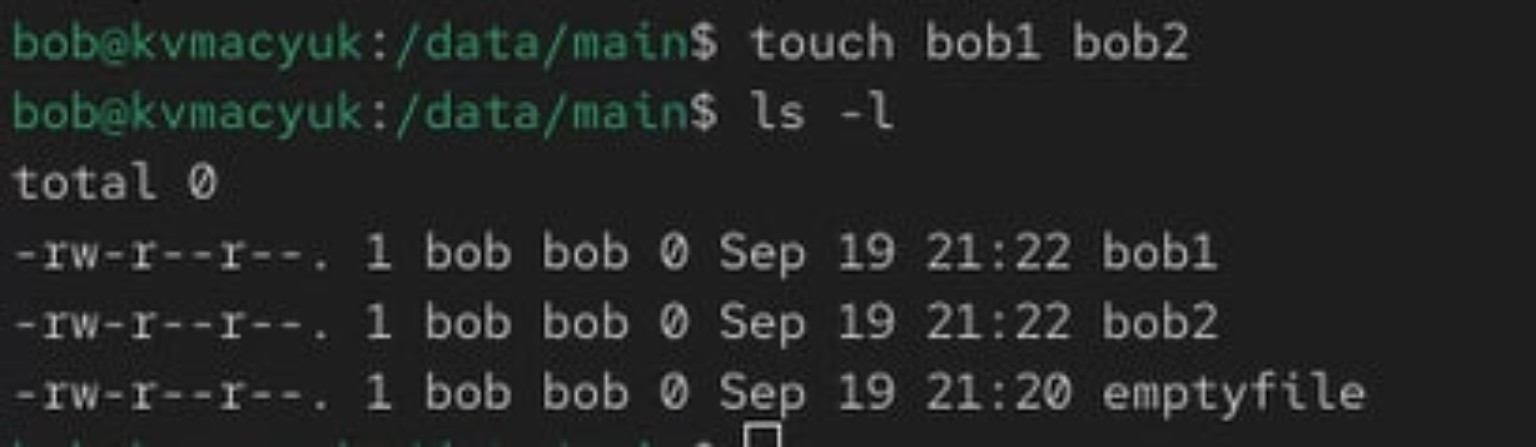
\includegraphics[width=0.85\linewidth,height=\textheight,keepaspectratio]{image/14.jpg}

}

\caption{\label{fig-014}Создание и проверка файлов bob1 и bob2}

\end{figure}%
\end{frame}

\begin{frame}[fragile]{Установка SGID и sticky bit}
\protect\phantomsection\label{ux443ux441ux442ux430ux43dux43eux432ux43aux430-sgid-ux438-sticky-bit}
\begin{itemize}
\tightlist
\item
  Пункт 6 раздела 3.3.2, терминал \texttt{root}
\end{itemize}

\begin{Shaded}
\begin{Highlighting}[]
\FunctionTok{chmod}\NormalTok{ g+s,o+t /data/main}
\end{Highlighting}
\end{Shaded}

\begin{itemize}
\tightlist
\item
  Установленным битам соответствует режим \texttt{3770}
\item
  Символьная запись: \texttt{drwxrws-\/-T}
\item
  SGID задаёт наследование группы, sticky bit ограничивает удаление
\end{itemize}
\end{frame}

\begin{frame}[fragile]{Значение специальных битов}
\protect\phantomsection\label{ux437ux43dux430ux447ux435ux43dux438ux435-ux441ux43fux435ux446ux438ux430ux43bux44cux43dux44bux445-ux431ux438ux442ux43eux432}
\begin{itemize}
\tightlist
\item
  \texttt{s} означает SGID при наличии группового права \texttt{x}
\item
  \texttt{T} означает sticky bit при отсутствии \texttt{x} у остальных
\item
  \texttt{o+t} не предоставляет остальным пользователям доступ
\item
  Группы уже существующих файлов \texttt{bob1} и \texttt{bob2} не
  меняются
\end{itemize}
\end{frame}

\begin{frame}{Установка SGID и sticky bit на /data/main}
\protect\phantomsection\label{ux443ux441ux442ux430ux43dux43eux432ux43aux430-sgid-ux438-sticky-bit-ux43dux430-datamain}
\begin{figure}

\centering{


\includegraphics[width=0.85\linewidth,height=\textheight,keepaspectratio]{image/15.jpg}

}

\caption{\label{fig-015}Установка SGID и sticky bit на /data/main}

\end{figure}%
\end{frame}

\begin{frame}[fragile]{Проверка наследования группы}
\protect\phantomsection\label{ux43fux440ux43eux432ux435ux440ux43aux430-ux43dux430ux441ux43bux435ux434ux43eux432ux430ux43dux438ux44f-ux433ux440ux443ux43fux43fux44b}
\begin{itemize}
\tightlist
\item
  Пункт 7 раздела 3.3.2
\item
  Терминал \texttt{alice}, текущий каталог \texttt{/data/main}
\end{itemize}

\begin{Shaded}
\begin{Highlighting}[]
\FunctionTok{touch}\NormalTok{ alice3 alice4}
\FunctionTok{ls} \AttributeTok{{-}l}
\end{Highlighting}
\end{Shaded}

\begin{itemize}
\tightlist
\item
  У новых файлов владелец \texttt{alice}, группа \texttt{main}
\item
  Группу задаёт SGID родительского каталога
\item
  Права файлов: \texttt{0644}; прежние файлы сохранили группу
  \texttt{bob}
\end{itemize}
\end{frame}

\begin{frame}{Наследование группы main файлами alice3 и alice4}
\protect\phantomsection\label{ux43dux430ux441ux43bux435ux434ux43eux432ux430ux43dux438ux435-ux433ux440ux443ux43fux43fux44b-main-ux444ux430ux439ux43bux430ux43cux438-alice3-ux438-alice4}
\begin{figure}

\centering{

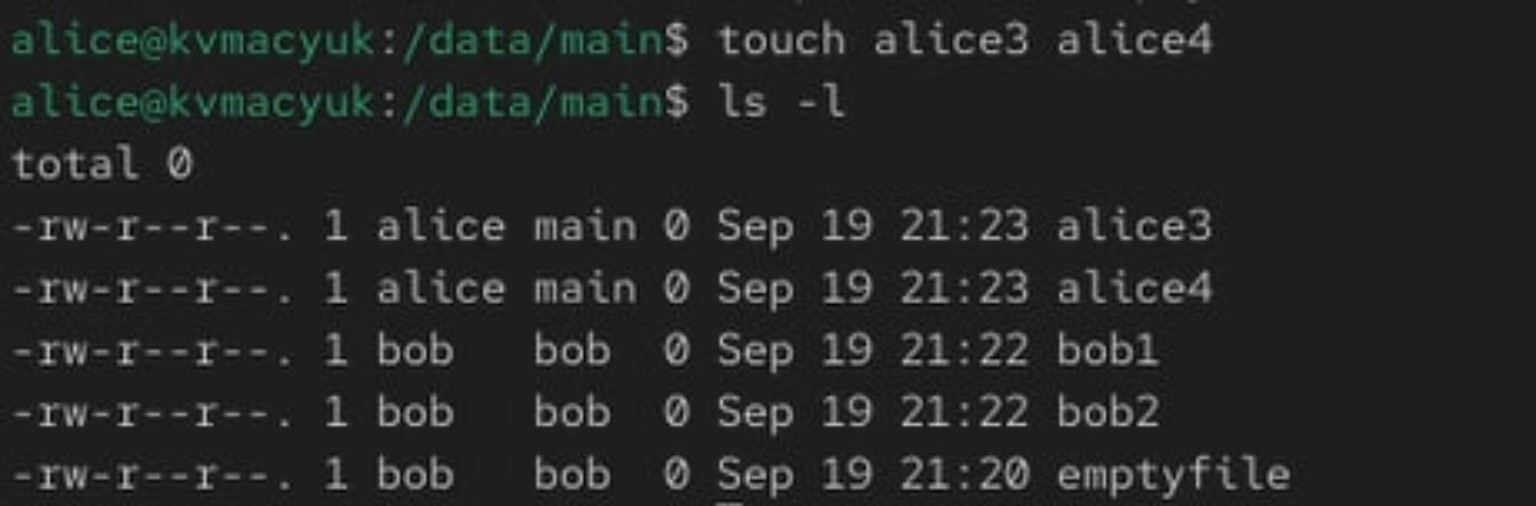
\includegraphics[width=0.85\linewidth,height=\textheight,keepaspectratio]{image/16.jpg}

}

\caption{\label{fig-016}Наследование группы main файлами alice3 и
alice4}

\end{figure}%
\end{frame}

\begin{frame}[fragile]{Проверка sticky bit}
\protect\phantomsection\label{ux43fux440ux43eux432ux435ux440ux43aux430-sticky-bit}
\begin{itemize}
\tightlist
\item
  Пункт 8 раздела 3.3.2, терминал \texttt{alice}
\end{itemize}

\begin{Shaded}
\begin{Highlighting}[]
\FunctionTok{rm} \AttributeTok{{-}rf}\NormalTok{ bob}\PreprocessorTok{*}
\end{Highlighting}
\end{Shaded}

\begin{itemize}
\tightlist
\item
  Удалить \texttt{bob1} и \texttt{bob2} не удалось
\item
  Оба файла остались в каталоге
\item
  Выведено сообщение \texttt{Operation\ not\ permitted}
\item
  Параметр \texttt{-f} не обходит проверку прав
\end{itemize}
\end{frame}

\begin{frame}[fragile]{Sticky bit и владелец каталога}
\protect\phantomsection\label{sticky-bit-ux438-ux432ux43bux430ux434ux435ux43bux435ux446-ux43aux430ux442ux430ux43bux43eux433ux430}
\begin{itemize}
\tightlist
\item
  Файлы \texttt{bob1} и \texttt{bob2} принадлежат \texttt{bob}
\item
  Каталог \texttt{/data/main} принадлежит \texttt{root}
\item
  \texttt{alice} не владеет ни этими файлами, ни каталогом
\item
  Свои файлы \texttt{alice} может удалять при имеющихся правах на
  каталог
\item
  Пояснение методички о владении каталогом пользователем \texttt{alice}
  не соответствует её командам
\end{itemize}
\end{frame}

\begin{frame}{Отказ alice в удалении файлов bob1 и bob2}
\protect\phantomsection\label{ux43eux442ux43aux430ux437-alice-ux432-ux443ux434ux430ux43bux435ux43dux438ux438-ux444ux430ux439ux43bux43eux432-bob1-ux438-bob2}
\begin{figure}

\centering{

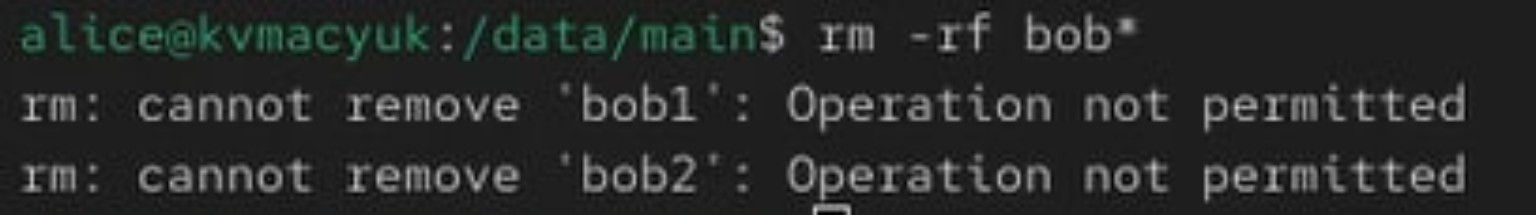
\includegraphics[width=0.85\linewidth,height=\textheight,keepaspectratio]{image/17.jpg}

}

\caption{\label{fig-017}Отказ alice в удалении файлов bob1 и bob2}

\end{figure}%
\end{frame}

\begin{frame}[fragile]{ACL: назначение прав каталогам}
\protect\phantomsection\label{acl-ux43dux430ux437ux43dux430ux447ux435ux43dux438ux435-ux43fux440ux430ux432-ux43aux430ux442ux430ux43bux43eux433ux430ux43c}
\begin{itemize}
\tightlist
\item
  Пункты 1--3 раздела 3.3.3, терминал \texttt{root}
\item
  Назначил дополнительные права группам и проверил ACL
\end{itemize}

\begin{Shaded}
\begin{Highlighting}[]
\ExtensionTok{setfacl} \AttributeTok{{-}m}\NormalTok{ g:third:rx /data/main}
\ExtensionTok{setfacl} \AttributeTok{{-}m}\NormalTok{ g:main:rx /data/third}
\ExtensionTok{getfacl}\NormalTok{ /data/main}
\ExtensionTok{getfacl}\NormalTok{ /data/third}
\end{Highlighting}
\end{Shaded}

\begin{itemize}
\tightlist
\item
  Дополнительные группы получают чтение и проход через каталог
\item
  Создание и удаление записей для них остаётся запрещённым
\end{itemize}
\end{frame}

\begin{frame}[fragile]{ACL каталога /data/main}
\protect\phantomsection\label{acl-ux43aux430ux442ux430ux43bux43eux433ux430-datamain}
\begin{Shaded}
\begin{Highlighting}[]
\NormalTok{user::rwx}
\NormalTok{group::rwx}
\NormalTok{group:third:r{-}x}
\NormalTok{mask::rwx}
\NormalTok{other::{-}{-}{-}}
\end{Highlighting}
\end{Shaded}

\begin{itemize}
\tightlist
\item
  \texttt{group::rwx} относится к группе-владельцу \texttt{main}
\item
  Запись \texttt{group:third:r-x} задаёт права группы \texttt{third}
\item
  SGID и sticky bit сохраняются
\end{itemize}
\end{frame}

\begin{frame}[fragile]{ACL каталога /data/third}
\protect\phantomsection\label{acl-ux43aux430ux442ux430ux43bux43eux433ux430-datathird}
\begin{Shaded}
\begin{Highlighting}[]
\NormalTok{user::rwx}
\NormalTok{group::rwx}
\NormalTok{group:main:r{-}x}
\NormalTok{mask::rwx}
\NormalTok{other::{-}{-}{-}}
\end{Highlighting}
\end{Shaded}

\begin{itemize}
\tightlist
\item
  \texttt{group::rwx} относится к группе-владельцу \texttt{third}
\item
  Запись \texttt{group:main:r-x} задаёт права группы \texttt{main}
\end{itemize}
\end{frame}

\begin{frame}[fragile]{Назначение ACL и исправление пути /data/thir}
\protect\phantomsection\label{ux43dux430ux437ux43dux430ux447ux435ux43dux438ux435-acl-ux438-ux438ux441ux43fux440ux430ux432ux43bux435ux43dux438ux435-ux43fux443ux442ux438-datathir}
\begin{figure}

\centering{

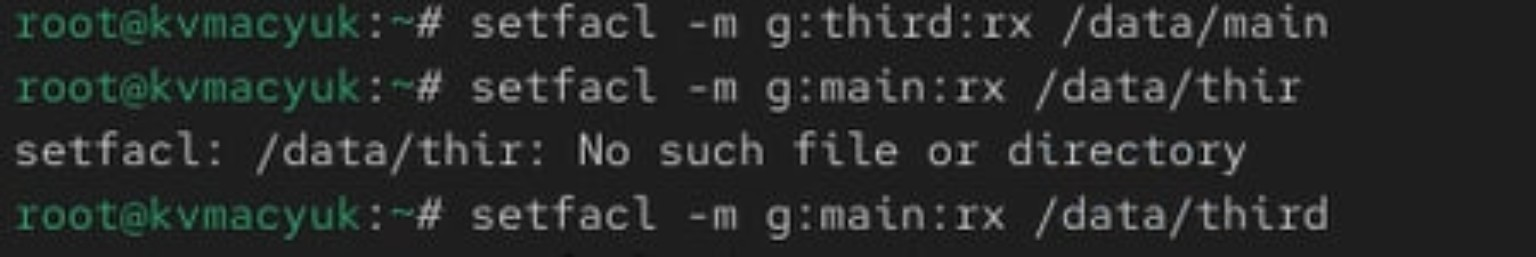
\includegraphics[width=0.85\linewidth,height=\textheight,keepaspectratio]{image/18.jpg}

}

\caption{\label{fig-018}Назначение ACL и исправление пути /data/thir}

\end{figure}%

\begin{itemize}
\tightlist
\item
  Опечатка \texttt{/data/thir} исправлена на \texttt{/data/third}
\end{itemize}
\end{frame}

\begin{frame}{Назначение ACL: повтор скриншота 18}
\protect\phantomsection\label{ux43dux430ux437ux43dux430ux447ux435ux43dux438ux435-acl-ux43fux43eux432ux442ux43eux440-ux441ux43aux440ux438ux43dux448ux43eux442ux430-18}
\begin{figure}

\centering{

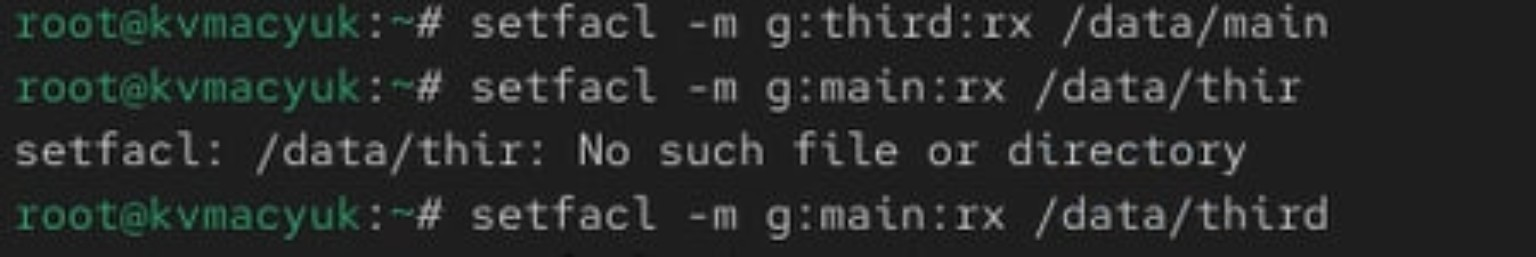
\includegraphics[width=0.85\linewidth,height=\textheight,keepaspectratio]{image/19.jpg}

}

\caption{\label{fig-019}Назначение ACL: повтор скриншота 18}

\end{figure}%

\begin{itemize}
\tightlist
\item
  В исходных материалах повторяется тот же скриншот
\end{itemize}
\end{frame}

\begin{frame}{Проверка ACL каталогов /data/main и /data/third}
\protect\phantomsection\label{ux43fux440ux43eux432ux435ux440ux43aux430-acl-ux43aux430ux442ux430ux43bux43eux433ux43eux432-datamain-ux438-datathird}
\begin{figure}

\centering{

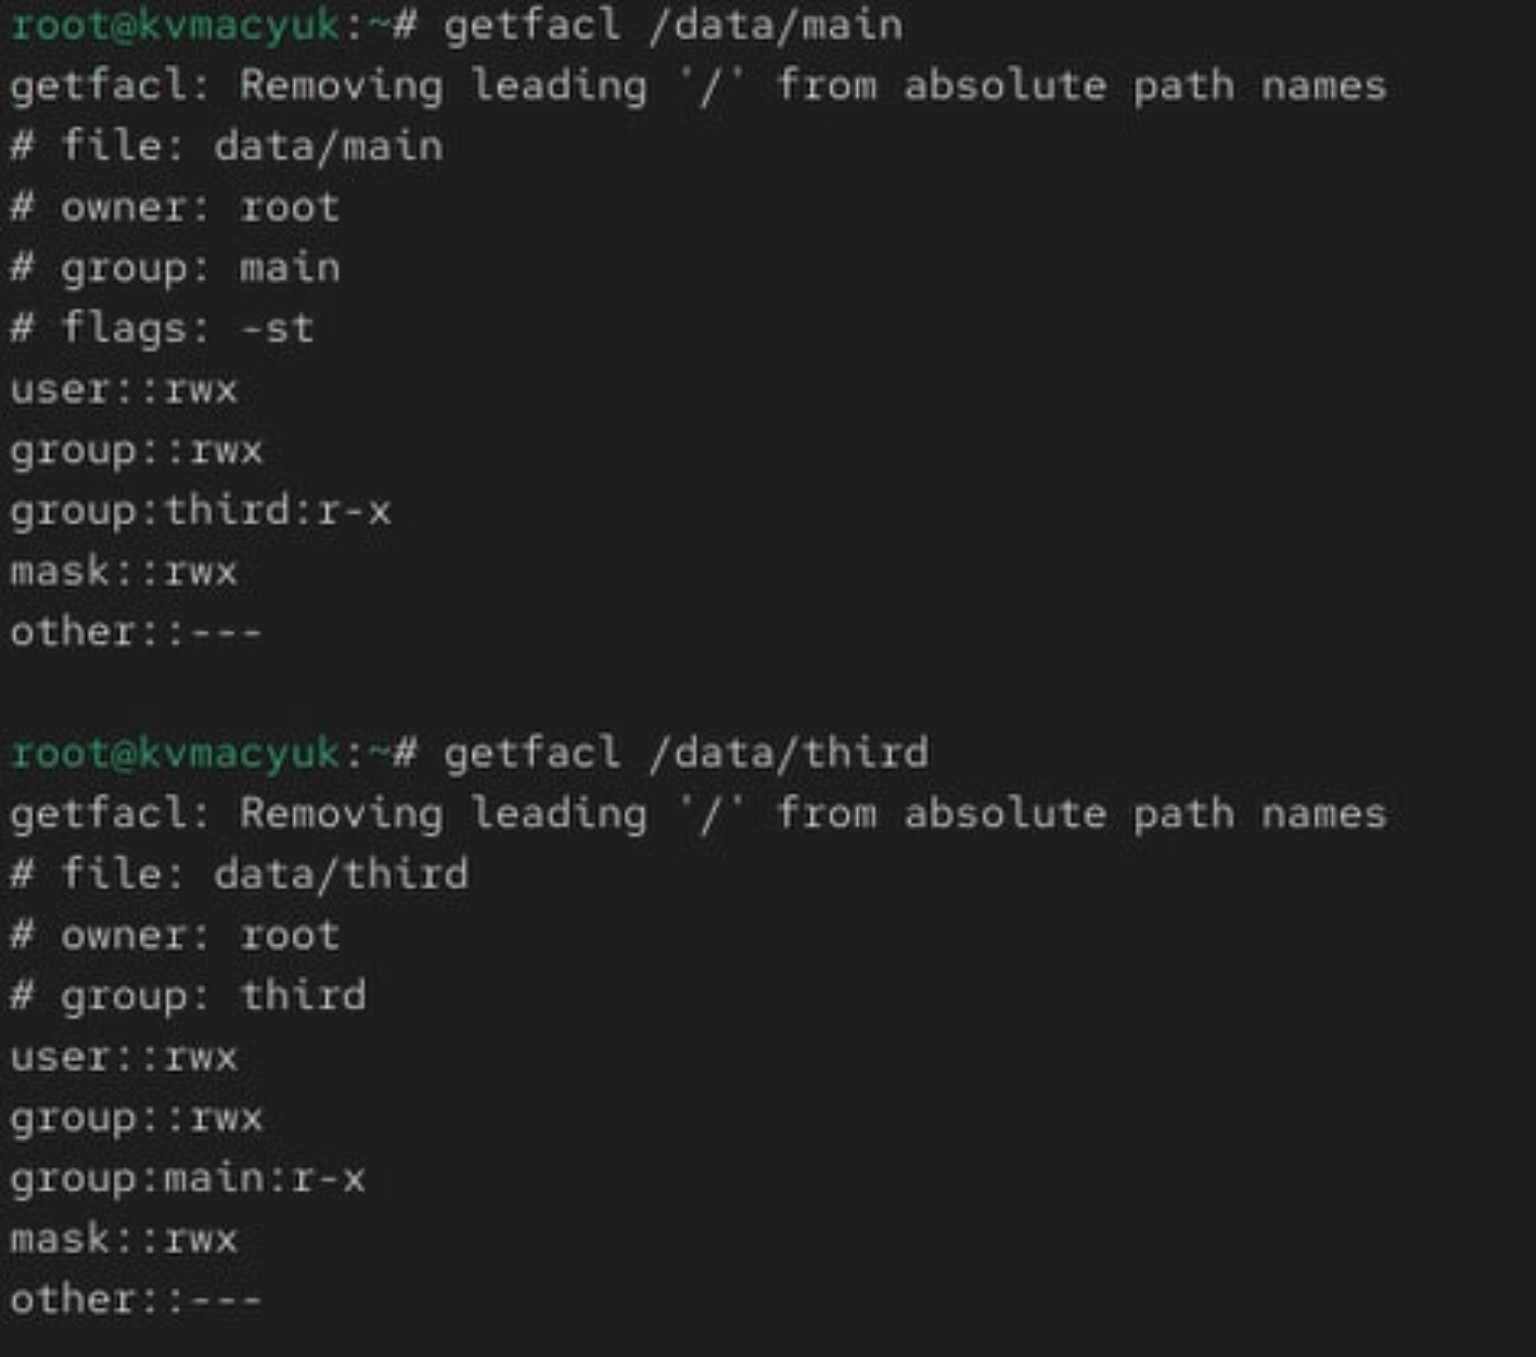
\includegraphics[width=\linewidth,height=0.68\textheight,keepaspectratio]{image/20.jpg}

}

\caption{\label{fig-020}Проверка ACL каталогов /data/main и /data/third}

\end{figure}%
\end{frame}

\begin{frame}[fragile]{Файлы newfile1 до настройки наследования}
\protect\phantomsection\label{ux444ux430ux439ux43bux44b-newfile1-ux434ux43e-ux43dux430ux441ux442ux440ux43eux439ux43aux438-ux43dux430ux441ux43bux435ux434ux43eux432ux430ux43dux438ux44f}
\begin{itemize}
\tightlist
\item
  Пункт 4 раздела 3.3.3, терминал \texttt{root}
\end{itemize}

\begin{Shaded}
\begin{Highlighting}[]
\FunctionTok{touch}\NormalTok{ /data/main/newfile1}
\ExtensionTok{getfacl}\NormalTok{ /data/main/newfile1}
\FunctionTok{touch}\NormalTok{ /data/third/newfile1}
\ExtensionTok{getfacl}\NormalTok{ /data/third/newfile1}
\end{Highlighting}
\end{Shaded}

\begin{itemize}
\tightlist
\item
  ACL доступа каталога сама по себе не наследуется
\item
  У файлов не появляются именованные записи для дополнительных групп
\end{itemize}
\end{frame}

\begin{frame}[fragile]{Владельцы и группы файлов newfile1}
\protect\phantomsection\label{ux432ux43bux430ux434ux435ux43bux44cux446ux44b-ux438-ux433ux440ux443ux43fux43fux44b-ux444ux430ux439ux43bux43eux432-newfile1}
{\def\LTcaptype{none} % do not increment counter
\begin{longtable}[]{@{}lll@{}}
\toprule\noalign{}
Файл & Владелец & Группа \\
\midrule\noalign{}
\endhead
\texttt{/data/main/newfile1} & \texttt{root} & \texttt{main} \\
\texttt{/data/third/newfile1} & \texttt{root} & \texttt{root} \\
\bottomrule\noalign{}
\end{longtable}
}

\begin{itemize}
\tightlist
\item
  В \texttt{/data/main} группу задаёт установленный SGID
\item
  В \texttt{/data/third} SGID отсутствует
\item
  Владельцы и группы подтверждены выводом \texttt{getfacl}
\end{itemize}
\end{frame}

\begin{frame}[fragile]{Права файлов newfile1}
\protect\phantomsection\label{ux43fux440ux430ux432ux430-ux444ux430ux439ux43bux43eux432-newfile1}
\begin{itemize}
\tightlist
\item
  Оба файла получили фактический режим \texttt{0644}
\end{itemize}

\begin{Shaded}
\begin{Highlighting}[]
\NormalTok{user::rw{-}}
\NormalTok{group::r{-}{-}}
\NormalTok{other::r{-}{-}}
\end{Highlighting}
\end{Shaded}

\begin{itemize}
\tightlist
\item
  \texttt{touch} запрашивает режим \texttt{0666}
\item
  Без ACL по умолчанию применяется
  \texttt{0666\ \&\ \textasciitilde{}umask}
\item
  Режим \texttt{0644} соответствует, в частности, маске \texttt{0022}
\item
  Право выполнения у обычного нового файла не появляется
\end{itemize}
\end{frame}

\begin{frame}{ACL файла /data/main/newfile1}
\protect\phantomsection\label{acl-ux444ux430ux439ux43bux430-datamainnewfile1}
\begin{figure}

\centering{

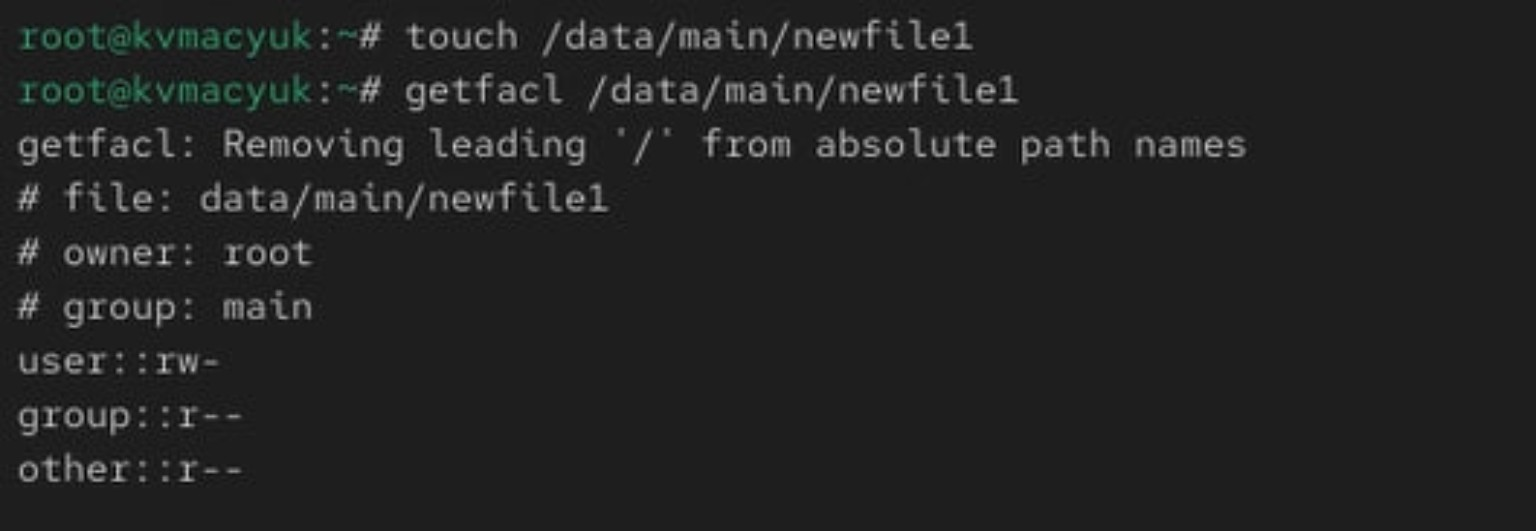
\includegraphics[width=0.85\linewidth,height=\textheight,keepaspectratio]{image/21.jpg}

}

\caption{\label{fig-021}ACL файла /data/main/newfile1}

\end{figure}%
\end{frame}

\begin{frame}{ACL файла /data/third/newfile1}
\protect\phantomsection\label{acl-ux444ux430ux439ux43bux430-datathirdnewfile1}
\begin{figure}

\centering{

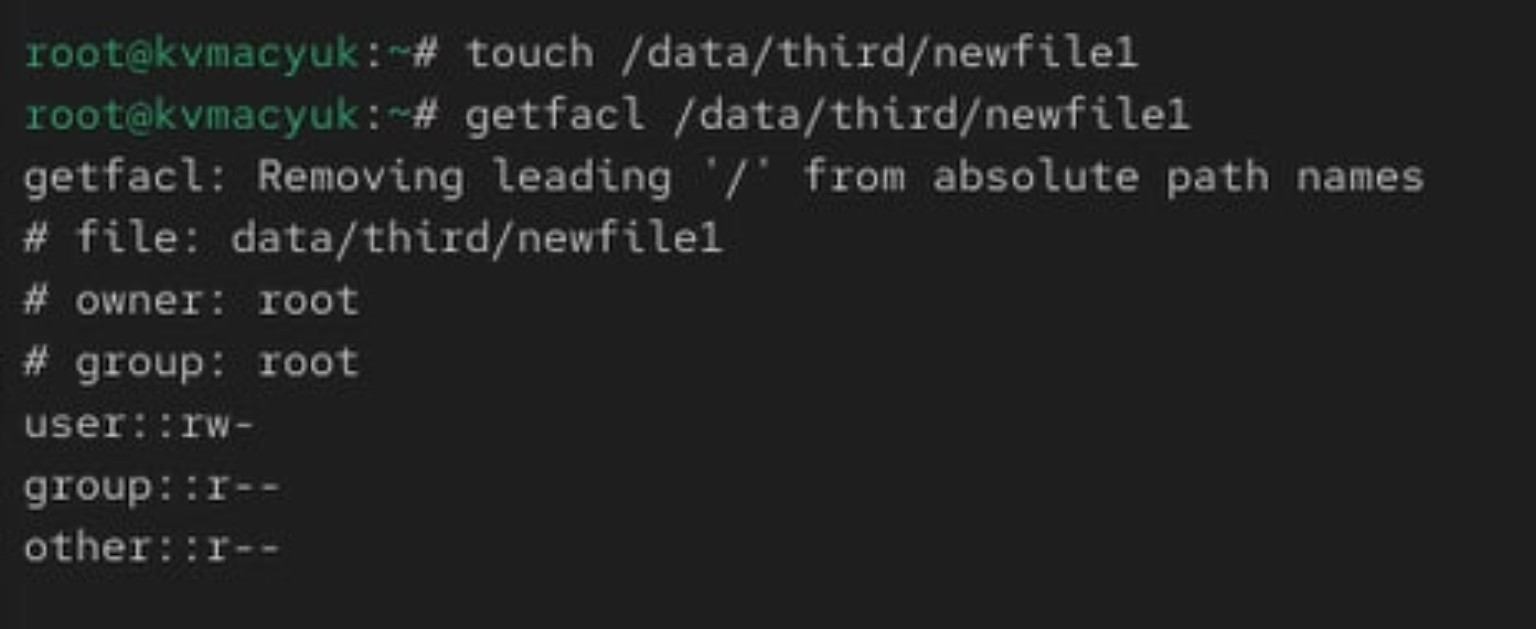
\includegraphics[width=0.85\linewidth,height=\textheight,keepaspectratio]{image/22.jpg}

}

\caption{\label{fig-022}ACL файла /data/third/newfile1}

\end{figure}%
\end{frame}

\begin{frame}[fragile]{Настройка ACL по умолчанию}
\protect\phantomsection\label{ux43dux430ux441ux442ux440ux43eux439ux43aux430-acl-ux43fux43e-ux443ux43cux43eux43bux447ux430ux43dux438ux44e}
\begin{itemize}
\tightlist
\item
  Пункты 5--6 раздела 3.3.3, терминал \texttt{root}
\end{itemize}

\begin{Shaded}
\begin{Highlighting}[]
\ExtensionTok{setfacl} \AttributeTok{{-}m}\NormalTok{ d:g:third:rwx /data/main}
\ExtensionTok{setfacl} \AttributeTok{{-}m}\NormalTok{ d:g:main:rwx /data/third}
\end{Highlighting}
\end{Shaded}

\begin{itemize}
\tightlist
\item
  Префикс \texttt{d:} обозначает ACL по умолчанию
\item
  \texttt{setfacl} дополняет недостающие базовые записи
\end{itemize}
\end{frame}

\begin{frame}[fragile]{Состав ACL по умолчанию для /data/main}
\protect\phantomsection\label{ux441ux43eux441ux442ux430ux432-acl-ux43fux43e-ux443ux43cux43eux43bux447ux430ux43dux438ux44e-ux434ux43bux44f-datamain}
\begin{Shaded}
\begin{Highlighting}[]
\NormalTok{default:user::rwx}
\NormalTok{default:group::rwx}
\NormalTok{default:group:third:rwx}
\NormalTok{default:mask::rwx}
\NormalTok{default:other::{-}{-}{-}}
\end{Highlighting}
\end{Shaded}

\begin{itemize}
\tightlist
\item
  Показана конфигурация, заданная выполненной командой
\item
  Новые объекты наследуют запись для группы \texttt{third}
\item
  ACL доступа самого каталога сохраняется
\end{itemize}
\end{frame}

\begin{frame}[fragile]{Состав ACL по умолчанию для /data/third}
\protect\phantomsection\label{ux441ux43eux441ux442ux430ux432-acl-ux43fux43e-ux443ux43cux43eux43bux447ux430ux43dux438ux44e-ux434ux43bux44f-datathird}
\begin{Shaded}
\begin{Highlighting}[]
\NormalTok{default:user::rwx}
\NormalTok{default:group::rwx}
\NormalTok{default:group:main:rwx}
\NormalTok{default:mask::rwx}
\NormalTok{default:other::{-}{-}{-}}
\end{Highlighting}
\end{Shaded}

\begin{itemize}
\tightlist
\item
  Показана конфигурация, заданная выполненной командой
\item
  Новые объекты наследуют запись для группы \texttt{main}
\item
  Ранее созданные файлы \texttt{newfile1} не изменяются
\end{itemize}
\end{frame}

\begin{frame}{ACL по умолчанию для /data/main}
\protect\phantomsection\label{acl-ux43fux43e-ux443ux43cux43eux43bux447ux430ux43dux438ux44e-ux434ux43bux44f-datamain}
\begin{figure}

\centering{

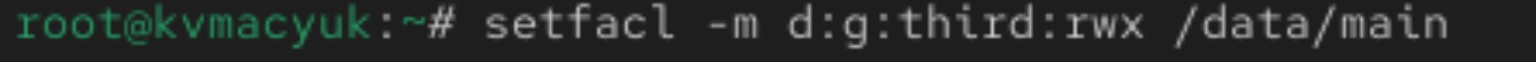
\includegraphics[width=0.85\linewidth,height=\textheight,keepaspectratio]{image/23.png}

}

\caption{\label{fig-023}ACL по умолчанию для /data/main}

\end{figure}%
\end{frame}

\begin{frame}{ACL по умолчанию для /data/third}
\protect\phantomsection\label{acl-ux43fux43e-ux443ux43cux43eux43bux447ux430ux43dux438ux44e-ux434ux43bux44f-datathird}
\begin{figure}

\centering{

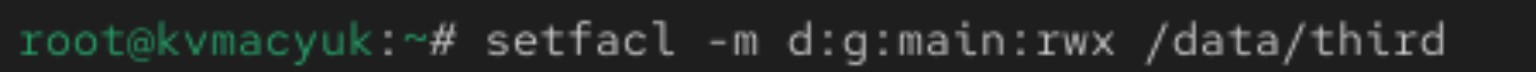
\includegraphics[width=0.85\linewidth,height=\textheight,keepaspectratio]{image/24.png}

}

\caption{\label{fig-024}ACL по умолчанию для /data/third}

\end{figure}%
\end{frame}

\begin{frame}[fragile]{Создание файлов newfile2}
\protect\phantomsection\label{ux441ux43eux437ux434ux430ux43dux438ux435-ux444ux430ux439ux43bux43eux432-newfile2}
\begin{itemize}
\tightlist
\item
  Пункт 7 раздела 3.3.3, терминал \texttt{root}
\end{itemize}

\begin{Shaded}
\begin{Highlighting}[]
\FunctionTok{touch}\NormalTok{ /data/main/newfile2}
\ExtensionTok{getfacl}\NormalTok{ /data/main/newfile2}
\FunctionTok{touch}\NormalTok{ /data/third/newfile2}
\ExtensionTok{getfacl}\NormalTok{ /data/third/newfile2}
\end{Highlighting}
\end{Shaded}

\begin{itemize}
\tightlist
\item
  Новые файлы наследуют ACL по умолчанию
\item
  Эффективные права ограничиваются режимом создания файла
\end{itemize}
\end{frame}

\begin{frame}[fragile]{ACL /data/main/newfile2}
\protect\phantomsection\label{acl-datamainnewfile2}
\begin{Shaded}
\begin{Highlighting}[]
\NormalTok{user::rw{-}}
\NormalTok{group::rwx        \#effective:rw{-}}
\NormalTok{group:third:rwx   \#effective:rw{-}}
\NormalTok{mask::rw{-}}
\NormalTok{other::{-}{-}{-}}
\end{Highlighting}
\end{Shaded}

\begin{itemize}
\tightlist
\item
  Владелец: \texttt{root}, группа: \texttt{main}
\item
  Группа \texttt{third} получает эффективные права \texttt{rw-}
\end{itemize}
\end{frame}

\begin{frame}[fragile]{ACL /data/third/newfile2}
\protect\phantomsection\label{acl-datathirdnewfile2}
\begin{Shaded}
\begin{Highlighting}[]
\NormalTok{user::rw{-}}
\NormalTok{group::rwx       \#effective:rw{-}}
\NormalTok{group:main:rwx   \#effective:rw{-}}
\NormalTok{mask::rw{-}}
\NormalTok{other::{-}{-}{-}}
\end{Highlighting}
\end{Shaded}

\begin{itemize}
\tightlist
\item
  По выводу \texttt{getfacl} владелец и группа: \texttt{root}
\item
  Группа \texttt{main} получает \texttt{rw-} через именованную запись
  ACL
\item
  Группа-владелец файла при этом не меняется
\end{itemize}
\end{frame}

\begin{frame}[fragile]{Маска ACL и режим создания файла}
\protect\phantomsection\label{ux43cux430ux441ux43aux430-acl-ux438-ux440ux435ux436ux438ux43c-ux441ux43eux437ux434ux430ux43dux438ux44f-ux444ux430ux439ux43bux430}
\begin{itemize}
\tightlist
\item
  \texttt{touch} запрашивает режим \texttt{0666}, без права выполнения
\item
  Поэтому маска нового файла равна \texttt{rw-}
\item
  Запись \texttt{rwx} ограничивается маской до эффективных \texttt{rw-}
\item
  Этим ACL соответствует режим \texttt{0660}: \texttt{-rw-rw-\/-\/-\/-+}
\item
  Знак \texttt{+} указывает на расширенную ACL
\end{itemize}
\end{frame}

\begin{frame}[fragile]{ACL по умолчанию и umask}
\protect\phantomsection\label{acl-ux43fux43e-ux443ux43cux43eux43bux447ux430ux43dux438ux44e-ux438-umask}
\begin{itemize}
\tightlist
\item
  При наличии ACL по умолчанию новый объект наследует её
\item
  Унаследованные права ограничиваются режимом, который запросило
  приложение
\item
  Правило \texttt{0666\ \&\ \textasciitilde{}umask} относится к случаю
  без ACL по умолчанию
\item
  Поэтому права \texttt{newfile1} и \texttt{newfile2} формируются по
  разным правилам
\end{itemize}
\end{frame}

\begin{frame}{Наследованная ACL файла /data/main/newfile2}
\protect\phantomsection\label{ux43dux430ux441ux43bux435ux434ux43eux432ux430ux43dux43dux430ux44f-acl-ux444ux430ux439ux43bux430-datamainnewfile2}
\begin{figure}

\centering{

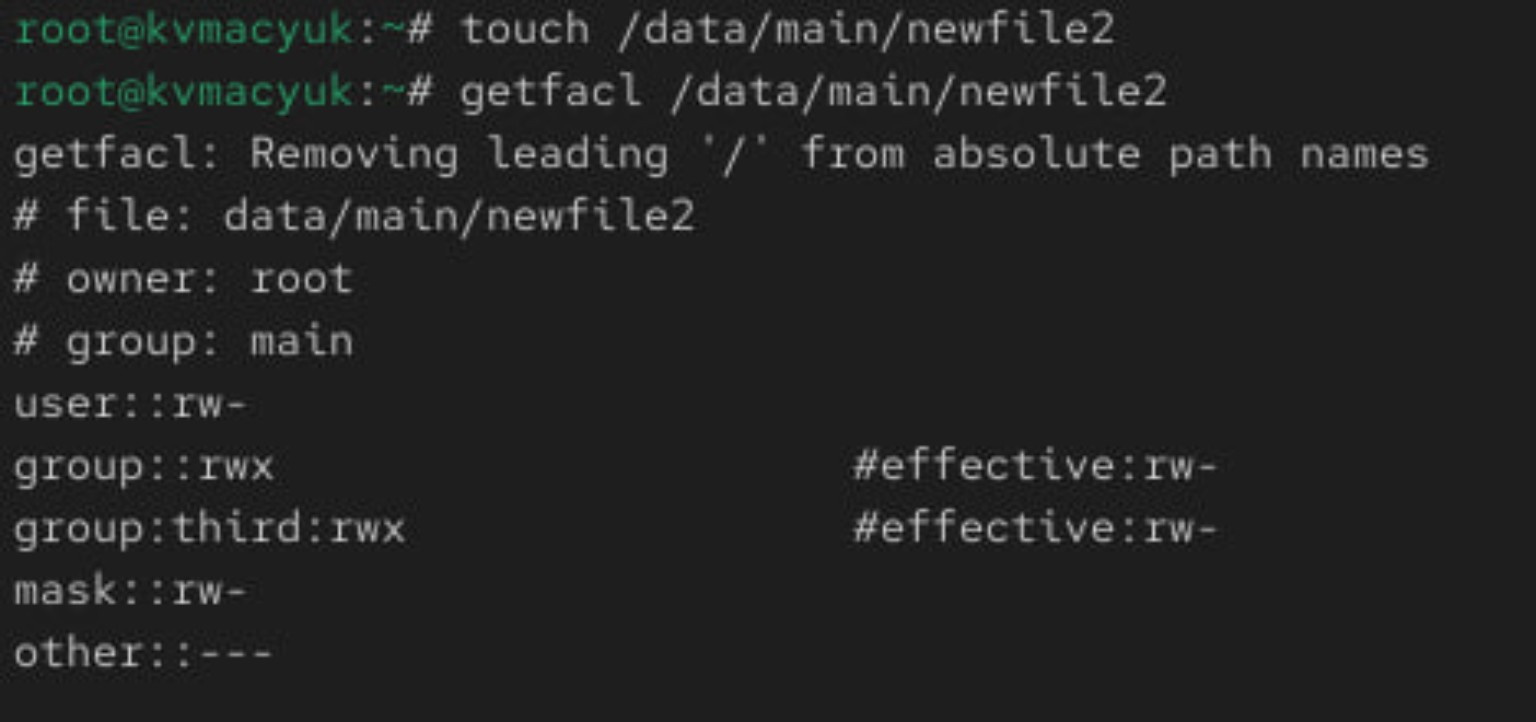
\includegraphics[width=0.85\linewidth,height=\textheight,keepaspectratio]{image/25.jpg}

}

\caption{\label{fig-025}Наследованная ACL файла /data/main/newfile2}

\end{figure}%
\end{frame}

\begin{frame}{Наследованная ACL файла /data/third/newfile2}
\protect\phantomsection\label{ux43dux430ux441ux43bux435ux434ux43eux432ux430ux43dux43dux430ux44f-acl-ux444ux430ux439ux43bux430-datathirdnewfile2}
\begin{figure}

\centering{

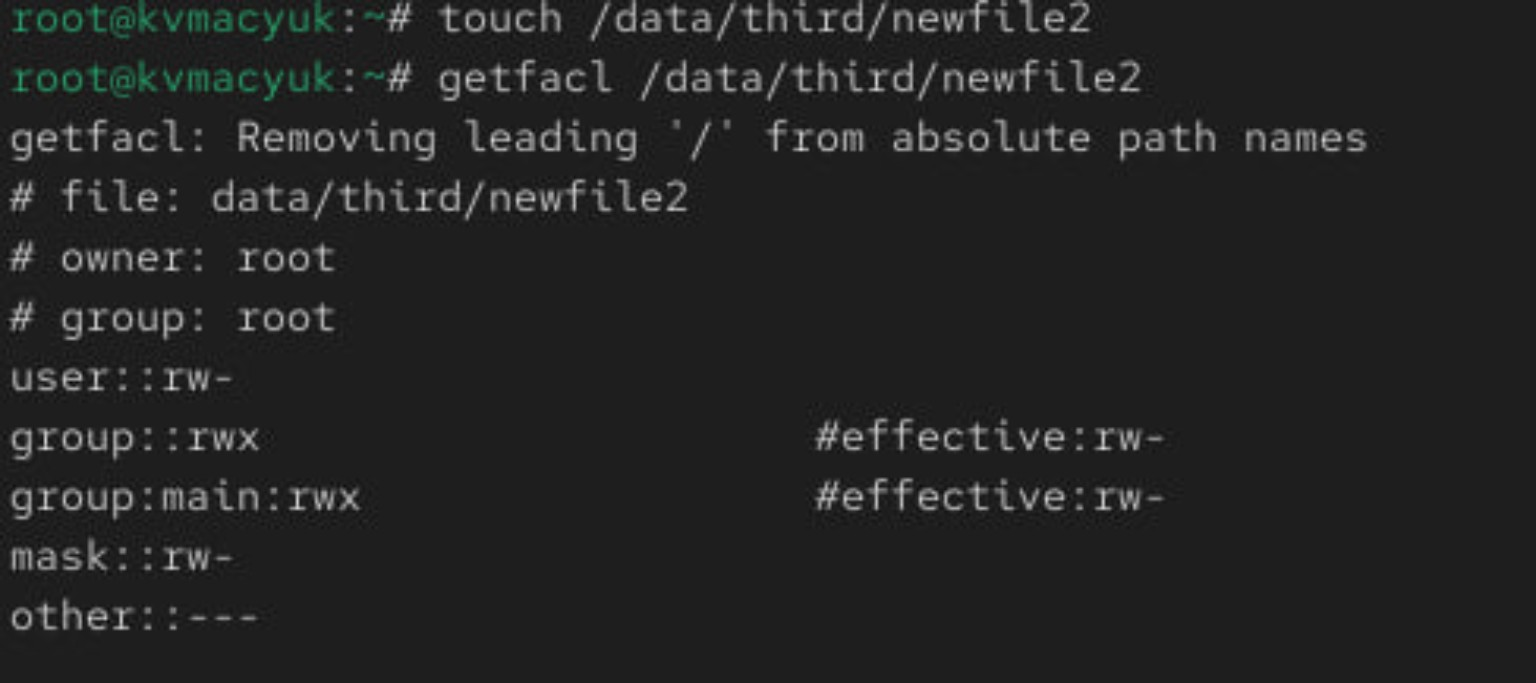
\includegraphics[width=0.85\linewidth,height=\textheight,keepaspectratio]{image/26.jpg}

}

\caption{\label{fig-026}Наследованная ACL файла /data/third/newfile2}

\end{figure}%
\end{frame}

\begin{frame}[fragile]{Проверка доступа пользователя carol}
\protect\phantomsection\label{ux43fux440ux43eux432ux435ux440ux43aux430-ux434ux43eux441ux442ux443ux43fux430-ux43fux43eux43bux44cux437ux43eux432ux430ux442ux435ux43bux44f-carol}
\begin{itemize}
\tightlist
\item
  Пункт 8 раздела 3.3.3, новый терминал
\item
  Проверки относятся к \texttt{/data/main}, как в командах методички
\end{itemize}

\begin{Shaded}
\begin{Highlighting}[]
\FunctionTok{su} \AttributeTok{{-}}\NormalTok{ carol}
\FunctionTok{rm}\NormalTok{ /data/main/newfile1}
\FunctionTok{rm}\NormalTok{ /data/main/newfile2}
\BuiltInTok{echo} \StringTok{"Hello, world"} \OperatorTok{\textgreater{}\textgreater{}}\NormalTok{ /data/main/newfile1}
\BuiltInTok{echo} \StringTok{"Hello, world"} \OperatorTok{\textgreater{}\textgreater{}}\NormalTok{ /data/main/newfile2}
\end{Highlighting}
\end{Shaded}
\end{frame}

\begin{frame}[fragile]{Результаты проверок carol}
\protect\phantomsection\label{ux440ux435ux437ux443ux43bux44cux442ux430ux442ux44b-ux43fux440ux43eux432ux435ux440ux43eux43a-carol}
\begin{itemize}
\tightlist
\item
  У \texttt{newfile1} фактические права \texttt{0644}, у
  \texttt{newfile2} --- ACL для \texttt{third}
\item
  Оба файла находятся в \texttt{/data/main}
\end{itemize}

{\def\LTcaptype{none} % do not increment counter
\begin{longtable}[]{@{}lll@{}}
\toprule\noalign{}
Действие & \texttt{newfile1} & \texttt{newfile2} \\
\midrule\noalign{}
\endhead
Удаление & Отказ & Отказ \\
Добавление строки & Отказ & Успех \\
\bottomrule\noalign{}
\end{longtable}
}
\end{frame}

\begin{frame}[fragile]{Причина отказа в удалении}
\protect\phantomsection\label{ux43fux440ux438ux447ux438ux43dux430-ux43eux442ux43aux430ux437ux430-ux432-ux443ux434ux430ux43bux435ux43dux438ux438}
\begin{itemize}
\tightlist
\item
  У группы \texttt{third} на каталог \texttt{/data/main} есть только
  \texttt{r-x}
\item
  Для удаления записи файла нужны \texttt{w} и \texttt{x} на каталог
\item
  Права записи в сам файл для удаления недостаточно
\item
  Sticky bit также защищает файлы \texttt{root} от удаления
  пользователем \texttt{carol}
\item
  \texttt{carol} не владеет ни файлами, ни каталогом
\end{itemize}
\end{frame}

\begin{frame}[fragile]{Причина различий при записи}
\protect\phantomsection\label{ux43fux440ux438ux447ux438ux43dux430-ux440ux430ux437ux43bux438ux447ux438ux439-ux43fux440ux438-ux437ux430ux43fux438ux441ux438}
\begin{itemize}
\tightlist
\item
  У \texttt{newfile1} нет именованной ACL для \texttt{third}
\item
  При режиме \texttt{0644} запись разрешена только владельцу
  \texttt{root}
\item
  У \texttt{newfile2} запись \texttt{group:third:rwx} и маска
  \texttt{rw-}
\item
  Для изменения содержимого нужны проход по пути и право \texttt{w} на
  файл
\item
  Право \texttt{w} на родительский каталог при этом не требуется
\end{itemize}
\end{frame}

\begin{frame}[fragile]{Подтверждение успешной записи}
\protect\phantomsection\label{ux43fux43eux434ux442ux432ux435ux440ux436ux434ux435ux43dux438ux435-ux443ux441ux43fux435ux448ux43dux43eux439-ux437ux430ux43fux438ux441ux438}
\begin{Shaded}
\begin{Highlighting}[]
\FunctionTok{cat}\NormalTok{ /data/main/newfile2}
\end{Highlighting}
\end{Shaded}

\begin{Shaded}
\begin{Highlighting}[]
\NormalTok{Hello, world}
\end{Highlighting}
\end{Shaded}

\begin{itemize}
\tightlist
\item
  Добавление строки в \texttt{newfile1} завершилось отказом
\item
  В \texttt{newfile2} строка успешно записана и прочитана
\end{itemize}
\end{frame}

\begin{frame}{Отказ carol в удалении newfile1 и newfile2}
\protect\phantomsection\label{ux43eux442ux43aux430ux437-carol-ux432-ux443ux434ux430ux43bux435ux43dux438ux438-newfile1-ux438-newfile2}
\begin{figure}

\centering{

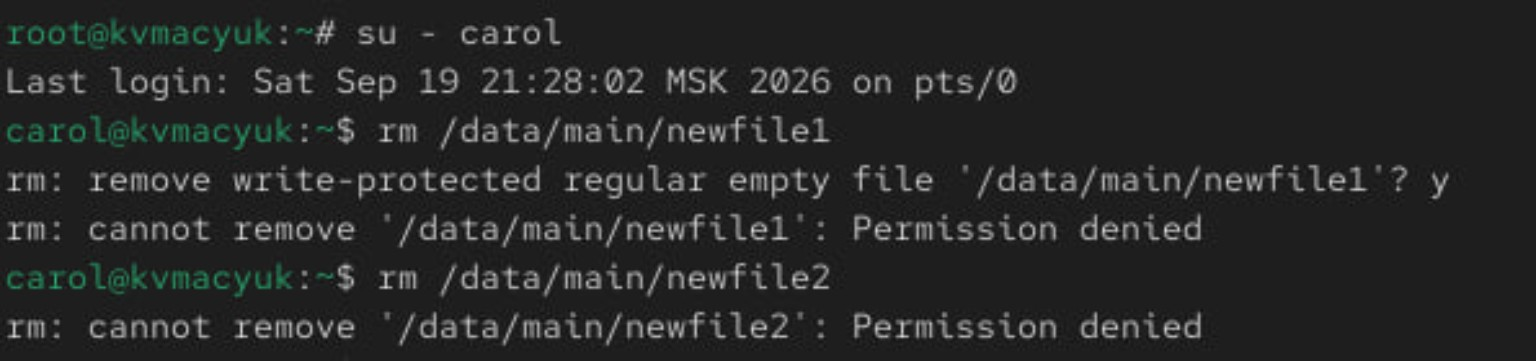
\includegraphics[width=0.85\linewidth,height=\textheight,keepaspectratio]{image/27.jpg}

}

\caption{\label{fig-027}Отказ carol в удалении newfile1 и newfile2}

\end{figure}%
\end{frame}

\begin{frame}{Проверка записи в файлы от имени carol}
\protect\phantomsection\label{ux43fux440ux43eux432ux435ux440ux43aux430-ux437ux430ux43fux438ux441ux438-ux432-ux444ux430ux439ux43bux44b-ux43eux442-ux438ux43cux435ux43dux438-carol}
\begin{figure}

\centering{

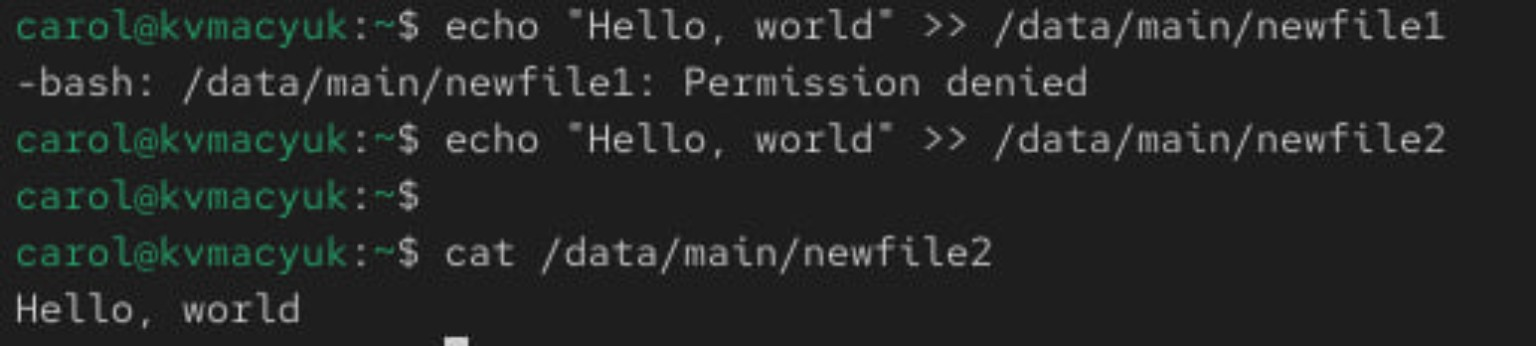
\includegraphics[width=0.85\linewidth,height=\textheight,keepaspectratio]{image/28.jpg}

}

\caption{\label{fig-028}Проверка записи в файлы от имени carol}

\end{figure}%
\end{frame}

\section{Ответы на контрольные
вопросы}\label{ux43eux442ux432ux435ux442ux44b-ux43dux430-ux43aux43eux43dux442ux440ux43eux43bux44cux43dux44bux435-ux432ux43eux43fux440ux43eux441ux44b}

\begin{frame}[fragile]{Вопрос 1}
\protect\phantomsection\label{ux432ux43eux43fux440ux43eux441-1}
\textbf{Как следует использовать команду chown, чтобы установить
владельца группы для файла? Приведите пример.}

\begin{Shaded}
\begin{Highlighting}[]
\FunctionTok{chown}\NormalTok{ :main /data/main/emptyfile}
\end{Highlighting}
\end{Shaded}

\begin{itemize}
\tightlist
\item
  Перед именем группы ставится двоеточие
\item
  Пользователь-владелец не меняется
\item
  Пример выполняется от имени \texttt{root}
\end{itemize}
\end{frame}

\begin{frame}[fragile]{Вопрос 2}
\protect\phantomsection\label{ux432ux43eux43fux440ux43eux441-2}
\textbf{С помощью какой команды можно найти все файлы, принадлежащие
конкретному пользователю? Приведите пример.}

\begin{Shaded}
\begin{Highlighting}[]
\FunctionTok{find}\NormalTok{ / }\AttributeTok{{-}type}\NormalTok{ f }\AttributeTok{{-}user}\NormalTok{ alice }\AttributeTok{{-}print}
\end{Highlighting}
\end{Shaded}

\begin{itemize}
\tightlist
\item
  \texttt{-user\ alice} выбирает владельца, \texttt{-type\ f} выбирает
  обычные файлы
\item
  Для обхода закрытых каталогов используется \texttt{root}
\item
  Для поиска объектов всех типов условие \texttt{-type\ f} убирают
\end{itemize}
\end{frame}

\begin{frame}[fragile]{Вопрос 3}
\protect\phantomsection\label{ux432ux43eux43fux440ux43eux441-3}
\textbf{Как применить разрешения на чтение, запись и выполнение для всех
файлов в каталоге /data для пользователей и владельцев групп, не
устанавливая никаких прав для других? Приведите пример.}

\begin{Shaded}
\begin{Highlighting}[]
\FunctionTok{chmod} \AttributeTok{{-}R}\NormalTok{ ug=rwx,o= /data}
\end{Highlighting}
\end{Shaded}

\begin{itemize}
\tightlist
\item
  \texttt{-R} применяет изменение рекурсивно
\item
  Владелец и группа получают \texttt{rwx}, остальные не получают прав
\end{itemize}
\end{frame}

\begin{frame}[fragile]{Вопрос 3: пояснение для ACL}
\protect\phantomsection\label{ux432ux43eux43fux440ux43eux441-3-ux43fux43eux44fux441ux43dux435ux43dux438ux435-ux434ux43bux44f-acl}
\begin{itemize}
\tightlist
\item
  Без расширенных ACL базовым правам соответствует \texttt{770}
\item
  При расширенной ACL групповые биты соответствуют её маске
\item
  \texttt{chmod} не удаляет именованные записи ACL
\end{itemize}
\end{frame}

\begin{frame}[fragile]{Вопрос 4}
\protect\phantomsection\label{ux432ux43eux43fux440ux43eux441-4}
\textbf{Какая команда позволяет добавить разрешение на выполнение для
файла, который необходимо сделать исполняемым?}

\begin{Shaded}
\begin{Highlighting}[]
\FunctionTok{chmod}\NormalTok{ u+x script.sh}
\end{Highlighting}
\end{Shaded}

\begin{itemize}
\tightlist
\item
  Команда добавляет выполнение владельцу файла
\item
  Остальные права сохраняются
\item
  Для всех трёх категорий применяется \texttt{chmod\ a+x\ script.sh}
\end{itemize}
\end{frame}

\begin{frame}[fragile]{Вопрос 5}
\protect\phantomsection\label{ux432ux43eux43fux440ux43eux441-5}
\textbf{Какая команда позволяет убедиться, что групповые разрешения для
всех новых файлов, создаваемых в каталоге, будут присвоены владельцу
группы этого каталога? Приведите пример.}

\begin{Shaded}
\begin{Highlighting}[]
\FunctionTok{chmod}\NormalTok{ g+s /data/main}
\end{Highlighting}
\end{Shaded}

\begin{itemize}
\tightlist
\item
  SGID обеспечивает наследование группы \texttt{main}
\item
  Конкретные права определяют режим создания, \texttt{umask} или ACL по
  умолчанию
\end{itemize}
\end{frame}

\begin{frame}[fragile]{Вопрос 6}
\protect\phantomsection\label{ux432ux43eux43fux440ux43eux441-6}
\textbf{Необходимо, чтобы пользователи могли удалять только те файлы,
владельцами которых они являются, или которые находятся в каталоге,
владельцами которого они являются. С помощью какой команды можно это
сделать? Приведите пример.}

\begin{Shaded}
\begin{Highlighting}[]
\FunctionTok{chmod}\NormalTok{ +t /data/main}
\end{Highlighting}
\end{Shaded}

\begin{itemize}
\tightlist
\item
  Sticky bit ограничивает удаление и переименование чужих файлов
\end{itemize}
\end{frame}

\begin{frame}{Вопрос 6: условия действия sticky bit}
\protect\phantomsection\label{ux432ux43eux43fux440ux43eux441-6-ux443ux441ux43bux43eux432ux438ux44f-ux434ux435ux439ux441ux442ux432ux438ux44f-sticky-bit}
\begin{itemize}
\tightlist
\item
  Для удаления нужны необходимые права на каталог
\item
  Обычный пользователь может удалить свой файл или файл в принадлежащем
  ему каталоге
\item
  Привилегированный пользователь может обходить это ограничение
\end{itemize}
\end{frame}

\begin{frame}[fragile]{Вопрос 7}
\protect\phantomsection\label{ux432ux43eux43fux440ux43eux441-7}
\textbf{Какая команда добавляет ACL, который предоставляет членам группы
права доступа на чтение для всех существующих файлов в текущем
каталоге?}

\begin{Shaded}
\begin{Highlighting}[]
\FunctionTok{find}\NormalTok{ . }\AttributeTok{{-}maxdepth}\NormalTok{ 1 }\AttributeTok{{-}type}\NormalTok{ f }\DataTypeTok{\textbackslash{}}
  \AttributeTok{{-}exec}\NormalTok{ setfacl }\AttributeTok{{-}m}\NormalTok{ g:third:r }\AttributeTok{{-}{-}}\NormalTok{ \{\} +}
\end{Highlighting}
\end{Shaded}

\begin{itemize}
\tightlist
\item
  Команда учитывает скрытые обычные файлы
\item
  \texttt{setfacl} без \texttt{-n} пересчитывает маску
\item
  Для доступа к файлам нужен проход через каталог
\end{itemize}
\end{frame}

\begin{frame}{Вопрос 8}
\protect\phantomsection\label{ux432ux43eux43fux440ux43eux441-8}
\textbf{Что нужно сделать для гарантии того, что члены группы получат
разрешения на чтение для всех файлов в текущем каталоге и во всех его
подкаталогах, а также для всех файлов, которые будут созданы в этом
каталоге в будущем? Приведите пример.}

\begin{itemize}
\tightlist
\item
  Назначить ACL существующим объектам
\item
  Настроить ACL по умолчанию для всех существующих каталогов
\end{itemize}
\end{frame}

\begin{frame}[fragile]{Вопрос 8: команды}
\protect\phantomsection\label{ux432ux43eux43fux440ux43eux441-8-ux43aux43eux43cux430ux43dux434ux44b}
\begin{Shaded}
\begin{Highlighting}[]
\ExtensionTok{setfacl} \AttributeTok{{-}R} \AttributeTok{{-}m}\NormalTok{ g:third:rX .}
\FunctionTok{find}\NormalTok{ . }\AttributeTok{{-}type}\NormalTok{ d }\DataTypeTok{\textbackslash{}}
  \AttributeTok{{-}exec}\NormalTok{ setfacl }\AttributeTok{{-}m}\NormalTok{ d:g:third:rx }\AttributeTok{{-}{-}}\NormalTok{ \{\} +}
\end{Highlighting}
\end{Shaded}

\begin{itemize}
\tightlist
\item
  Первая команда разрешает чтение существующих объектов
\item
  \texttt{X} добавляет проход каталогам и выполнение уже исполняемым
  файлам
\item
  Вторая команда задаёт наследование новым объектам
\item
  Новые подкаталоги тоже наследуют ACL по умолчанию
\end{itemize}
\end{frame}

\begin{frame}[fragile]{Вопрос 8: границы наследования}
\protect\phantomsection\label{ux432ux43eux43fux440ux43eux441-8-ux433ux440ux430ux43dux438ux446ux44b-ux43dux430ux441ux43bux435ux434ux43eux432ux430ux43dux438ux44f}
\begin{itemize}
\tightlist
\item
  Для обычного файла с режимом создания \texttt{0666} группа получает
  чтение
\item
  Для каталога с режимом создания \texttt{0777} группа получает
  \texttt{r-x}
\item
  Явно ограничительный режим, например \texttt{0600}, может урезать
  права
\item
  Владелец может впоследствии изменить ACL
\item
  Для доступа нужен проход по пути до текущего каталога
\end{itemize}
\end{frame}

\begin{frame}[fragile]{Вопрос 9}
\protect\phantomsection\label{ux432ux43eux43fux440ux43eux441-9}
\textbf{Какое значение umask нужно установить, чтобы «другие»
пользователи не получали какие-либо разрешения на новые файлы? Приведите
пример.}

\begin{Shaded}
\begin{Highlighting}[]
\BuiltInTok{umask}\NormalTok{ 0007}
\end{Highlighting}
\end{Shaded}

\begin{itemize}
\tightlist
\item
  Без ACL по умолчанию обычный файл получает \texttt{0660}, каталог
  получает \texttt{0770}
\item
  Последняя цифра \texttt{7} запрещает все права категории «остальные»
\item
  При ACL по умолчанию нужна запись \texttt{default:other::-\/-\/-}
\end{itemize}
\end{frame}

\begin{frame}[fragile]{Вопрос 10}
\protect\phantomsection\label{ux432ux43eux43fux440ux43eux441-10}
\textbf{Какая команда гарантирует, что никто не сможет удалить файл
myfile случайно?}

\begin{Shaded}
\begin{Highlighting}[]
\FunctionTok{chattr}\NormalTok{ +i myfile}
\end{Highlighting}
\end{Shaded}

\begin{itemize}
\tightlist
\item
  Команда выполняется от имени \texttt{root}
\item
  Нужна поддержка атрибута неизменяемости файловой системой
\item
  Атрибут \texttt{i} запрещает удаление, переименование и изменение
  файла
\item
  Привилегированный процесс может снять его: \texttt{chattr\ -i\ myfile}
\end{itemize}
\end{frame}

\section{Выводы}\label{ux432ux44bux432ux43eux434ux44b}

\begin{frame}[fragile]{Выводы}
\begin{itemize}
\tightlist
\item
  Режим \texttt{770} разделяет доступ групп \texttt{main} и
  \texttt{third}
\item
  SGID обеспечивает наследование группы новыми объектами
\item
  Sticky bit ограничивает удаление чужих файлов
\item
  ACL задаёт права дополнительных групп и наследование разрешений
\end{itemize}
\end{frame}

\begin{frame}[fragile]{Выводы: проверка результата}
\protect\phantomsection\label{ux432ux44bux432ux43eux434ux44b-ux43fux440ux43eux432ux435ux440ux43aux430-ux440ux435ux437ux443ux43bux44cux442ux430ux442ux430}
\begin{itemize}
\tightlist
\item
  Право изменять содержимое файла отличается от права удалить его запись
  из каталога
\item
  После настройки ACL \texttt{carol} успешно дописала строку в
  \texttt{/data/main/newfile2}
\item
  Удаление этого файла для \texttt{carol} остаётся запрещённым
\item
  Фактические результаты подтверждаются скриншотами Rocky Linux
\end{itemize}
\end{frame}

\section*{Список
литературы}\label{ux441ux43fux438ux441ux43eux43a-ux43bux438ux442ux435ux440ux430ux442ux443ux440ux44b}
\addcontentsline{toc}{section}{Список литературы}

\begin{frame}[fragile]{Методические указания}
\protect\phantomsection\label{ux43cux435ux442ux43eux434ux438ux447ux435ux441ux43aux438ux435-ux443ux43aux430ux437ux430ux43dux438ux44f}
\begin{itemize}
\tightlist
\item
  Кулябов Д. С., Королькова А. В. Основы администрирования операционных
  систем
\item
  Лабораторная работа № 3 «Настройка прав доступа»
\item
  Предоставленный файл \texttt{004-permissions.pdf}, с. 27--31
\end{itemize}
\end{frame}

\begin{frame}[fragile]{Справочные страницы Linux}
\protect\phantomsection\label{ux441ux43fux440ux430ux432ux43eux447ux43dux44bux435-ux441ux442ux440ux430ux43dux438ux446ux44b-linux}
\protect\phantomsection\label{refs}
\begin{CSLReferences}{0}{1}
\begin{itemize}
\tightlist
\item
  \texttt{chgrp(1)},
  \href{https://man7.org/linux/man-pages/man1/chmod.1.html}{chmod(1)}
\item
  \href{https://man7.org/linux/man-pages/man1/getfacl.1.html}{getfacl(1)},
  \href{https://man7.org/linux/man-pages/man1/setfacl.1.html}{setfacl(1)}
\item
  \href{https://man7.org/linux/man-pages/man5/acl.5.html}{acl(5)}
\item
  \href{https://man7.org/linux/man-pages/man1/chown.1.html}{chown(1)},
  \href{https://man7.org/linux/man-pages/man1/find.1.html}{find(1)}
\item
  \href{https://man7.org/linux/man-pages/man1/chattr.1.html}{chattr(1)}
\end{itemize}

\end{CSLReferences}
\end{frame}




\end{document}
